\documentclass[a4paper,10pt]{article}
\usepackage[utf8]{inputenc}
\usepackage{xspace}
\usepackage{url}
\usepackage{graphicx,graphics} 
\usepackage{color}
\usepackage{amsmath}
\usepackage{amsfonts}
\usepackage{amssymb}
\usepackage{amsthm}
\usepackage{algorithm}
\usepackage{algorithmic}
\usepackage{longtable}
\usepackage{complexity}
\usepackage{tkz-graph}
\usepackage{float}
\usepackage{setspace}
\renewcommand{\algorithmicrequire}{\textbf{Input:}}
\renewcommand{\algorithmicensure}{\textbf{Output:}}
\usepackage{authblk}
  
\graphicspath{{figures/}}
\makeatletter
\def\input@path{{figures/}}
\makeatother
\newcommand\rmatching{${\cal R}$-matching\xspace}
\newcommand\mdelay{$\cal M$-delay\xspace}
\newcommand\matchedgraph{{\bf matched graph}}
\newtheorem{proposition}{Proposition}
\newtheorem{theorem}{Theorem}

\setlength{\parskip}{1ex} % Espace entre les paragraphes

\newtheorem{fact}{Fact}
\newtheorem{lemma}[theorem]{Lemma}
\newtheorem{definition}{Definition}
\newtheorem{corollary}{Corollary}



\newcommand{\todo}[1]{{\color{red} TODO: {#1}}}


%opening
\title{Deterministic Scheduling of Periodic Messages in a Network}% by a SDN (deterministic) approach}
%\author{Dominique Barth - UVSQ ,Christian Cad�r� - UVSQ,Ma�l Guiraud - UVSQ,Olivier Marc� - Nokia Bell Labs France,Yann Strozecki - UVSQ}

\author[1]{Ma\"el Guiraud}
\author[1]{Dominique Barth}
\author[1]{Christian Cad\'er\'e}
\author[2]{Brice Leclerc}
\author[2]{Olivier Marc\'e}
\author[1]{Yann Strozecki}
\affil[1]{David Laboratory, UVSQ}
\affil[2]{Nokia Bell Labs France}

\begin{document}

\maketitle

\begin{abstract}
We study the sending of periodic messages in a graph following predefined paths, a problem arising from communication between radio antennas and their signal processing units located in distant data-centers. Messages must be sent deterministically to avoid collisions on the network and to minimize the latency. We prove that problems arising from this context are $\NP$-complete even for very restricted graphs. We then deal with the case of a star graph and for different regimes of the parameters we propose algorithms that are experimentally shown to work extremely well compared to traditional statistical multiplexing.
\end{abstract}


\section{Introduction}

Next generations of mobile network architectures evolve toward centralized radio network architectures or C-RAN, for Cloud Radio Access Network, to reduce energy consumption costs~\cite{mobile2011c}. The main challenge for this type of architecture is the latency in the transfer process between the Remote Radio Heads (RRHs) on the field and the Baseband Units (BBUs) in the cloud. The standard requires meeting time constraints for functions like HARQ (Hybrid Automatic Repeat reQuest) that needs to be processed in 1 to 10ms depending on targeted services~\cite{bouguen2012lte}. The specificity of the C-RAN context is not only the latency constraint, but also the periodicity of the data transfer between RRHs and BBUs.

 In this article, we study mechanisms to deal with the latency and periodicity constraints in the fronthaul network.  The current solution is to use stochastic multiplexing \todo{ref} with a traditional queue management in an optical network with a very large bandwidth to minimize latency. Here we propose to use a deterministic approach to schedule our periodic messages. This approach has gained some traction recently: Deterministic Networking is under standardization in IEEE 802.1 TSN group~\cite{finn-detnet-architecture-08}, as well at IETF DetNet working group~\cite{ieee802}. Several patents on concepts and mechanisms for DetNet have been already published, see for example~\cite{howe2005time,leclerc2016transmission}.

 
Let us expose briefly our model: the network topology is modeled by a directed weighted graph and a set of paths (routes) from source nodes (RRHs) to target nodes (BBUs). Time is discretized and a unit of time corresponds to the transmission of a minimal unit of data over the network.
 The process must be periodic, that is if we look at the network at times $t$ and $t+P$ where $P$ is the period, all messages are at the same position in the network. Moreover, we want to avoid any  buffering in internal nodes of the graph. Hence we need to design 
 a periodic process with no collision between messages. To ensure that this property is always true we propose a deterministic process.  We have two sets of parameters that we can choose when building a periodic sending process, called a \textbf{periodic assignment} in this article: the time at which each packet is sent by a RRH in each period and the waiting time in the BBU before the answer is sent back to the RRH. When building a periodic assignment, we must take into account the periodicity which makes many scheduling methods inapplicable. Not only a message must not collide with the other messages sent by the others BBU/RRH in the same period, but also in the previous and following periods. Moreover the latency must be minimized, that is the time 
 between the emission of a message and the complete return of its answer. It means that the only buffering we are allowed -- the waiting time before sending back the answer-- must be small, in particular when the route is long.
 
This problem may look like wormhole problems~\cite{cole1996benefit}, but here we want to minimize the time lost in buffers and not just avoid deadlocks, moreover the periodicity is not considered in wormhole problems. Several graph colorings have been introduced to model similar problems such as the allocation of frequencies~\cite{borndorfer1998frequency}, bandwidths~\cite{erlebach2001complexity} or routes~\cite{cole1996benefit} in a network or train schedules~\cite{strotmann2007railway}. Unfortunately, they do not take into account the periodicity of the scheduling and the associated problems are also $\NP$-complete. The only model which incorporates some periodicity is the circular coloring~\cite{zhou2013multiple, zhu2001circular,zhu2006recent} but is not expressive enough to capture our problem.


 In Sec.~\ref{sec:def} we propose a model of the network and the periodic sending of messages along its routes. 
 We then formalize our two problems of finding a periodic assignment for sending messages without collisions: PRA (sending of the message only) and PALL (sending of the message and answer).  
In Sec.~\ref{sec:complexity}, we prove that the problem PRA and PALL are $\NP$-hard and cannot be approximated even for very
restricted classes of graphs. 
Therefore in the next two sections, we study a simple but very common topology, that we call the
star topology, where all messages can collide on a single arc.
In Sec.\ref{sec:PAZL}, we study a variant of PALL called PAZL  where the waiting times must all be zero. We provide several algorithms, some of their theoretical properties and give experimental evidences that they find periodic assignments when the network is no too loaded. Finally in Sec.\ref{sec:PALL}, we propose algorithms for the general PALL problem and exhibit one which works extremely well in our experiments even in loaded networks. In particular we show that the deterministic communication schemes we design vastly outperform the traditional stochastic multiplexing with regards to latency. 


\section{Model and Problems}\label{sec:def}

  \subsection{Network modeling}
  

The network is modeled as a directed graph $G=(V,A)$. Each arc  $(u,v)$ in $A$ is labeled by an integer weight $\omega(u,v)$ which represents the time slots taken by a signal to go from $u$ to $v$ using this arc. A {\bf route} $r$ in $G$ is a path, that is sequence of consecutive arcs $a_0, \ldots , a_{k-1}$, with $a_i=(u_i,u_{i+1}) \in A$.  The {\bf latency} of a vertex $u_i$ in a path $r$, with $i \geq 1$, is defined by $\lambda(u_i,r)= \sum\limits_{0 \leq j <i} \omega(a_j)$. We also define $\lambda(u_0,r)=0$. The latency of the route $r$ is defined by $\lambda (r)= \lambda (u_k,r)$. \todo{remettre premier et dernier sommet disjoint ? 
V�rifier si c'est g�nant dans la suite, �a l'est un peu quand on d�finit le graphe symm�trique}
We denote by $\cal R$ a set of routes,  %in $G$ such that no two routes have the same first vertices or the same last vertices.
the pair $(G,\cal R)$ is called a {\bf routed network} and represents our telecommunication network.
The first vertex of a route models an antenna (RRH) and the last one a data-center (BBU) which processes the messages sent by the antenna.

%We denote by $\rho$ the bijection induced by ${\cal R}$, $\rho(s) = t$ if $s$ is the first vertex of a route $r$ and $t$ the last. 



   \subsection{Messages dynamic}
      
      Consider a route $r$, if a message is sent at time $m$ from $s$ the first vertex of $r$ then it will arrive at vertex $v$ in $r$ at time $m + \lambda(v,r)$. In our problem, we send one message on each route periodically and we denote the period by $P$.
      Periodicity means that if we look at the messages going through an edge between time $0$ and $P-1$, then we would observe the same messages in the same order and position between time $kP$ and $(k+1)P -1$ for all $k$. 
      Therefore, we will always consider a period of $P$ discrete slots of time at each edge to characterize the working of the network. We define the first time slot at which a message sent from the first vertex of $r$ will reach a vertex $v$ in $r$ by $t(v,r) = m + \lambda(v,r) \mod P$. 
      
      A message usually cannot be transported in a single time slot. We denote by $\tau$ the number 
      of \emph{consecutive slots} necessary to transmit a message. Let us call $[t(v,r)]_{P,\tau}$ the set of time slots used by route $r$ at vertex $v$ in a period $P$, that is $[t(v,r)]_{P,\tau} = \{t(v,r) + k \mod P \mid 0 \leq k < \tau \}$. Usually $P$ and $\tau$ will be clear from the context and we will denote $[t(v,r)]_{P,\tau}$ by $[t(v,r)]$.
      Let $r_1$ and $r_2$ be two routes, on which messages are sent at time $m_1$ and $m_2$ in their first vertex.
      We say that the two routes have a {\bf collision} if they share an arc of first vertex $v$ and $[t(v,r_{1})] \cap [t(v,r_{2})] \neq \emptyset$.
      
      A {\bf $(P,\tau)$-periodic assignment} of a routed network $(G,\cal R)$ is a sequence  ${\cal M}=(m_1, \ldots ,m_n)$ of $n$ integers that we call {\bf offsets}, with $n$ the number of routes in $\cal R$. The number $m_{i}$ represents the time at which a message is emitted at the first vertex of the route $r_{i}$. We will always consider that the $m_{i}$ are between $0$ and $P-1$. Moreover, \emph{no pair of routes must have a collision} in a $(P,\tau)$-periodic assignment.
      

%       Notice that the notion of $P$-periodic assignment \textbf{is not monotone} with regard to $P$. 
      As an example of a $(2,1)$-periodic assignment, let us consider a routed network 
      where all pairs of routes intersect at a different edge. It is easy to design such a network and an example is given in Fig.~\ref{fig:example}. We set $\tau = 1$ and the weights are chosen so that if $r_{i}$ and $r_{j}$ have $v$ as first common vertex then we have $\lambda(v,r_{i}) - \lambda(v,r_{j})=1$. There is a $(2,1)$-periodic assignment by setting all $m_{i}$ to $0$.

  
      \begin{figure}[ht]
      \begin{center}
          \scalebox{0.8}{
          
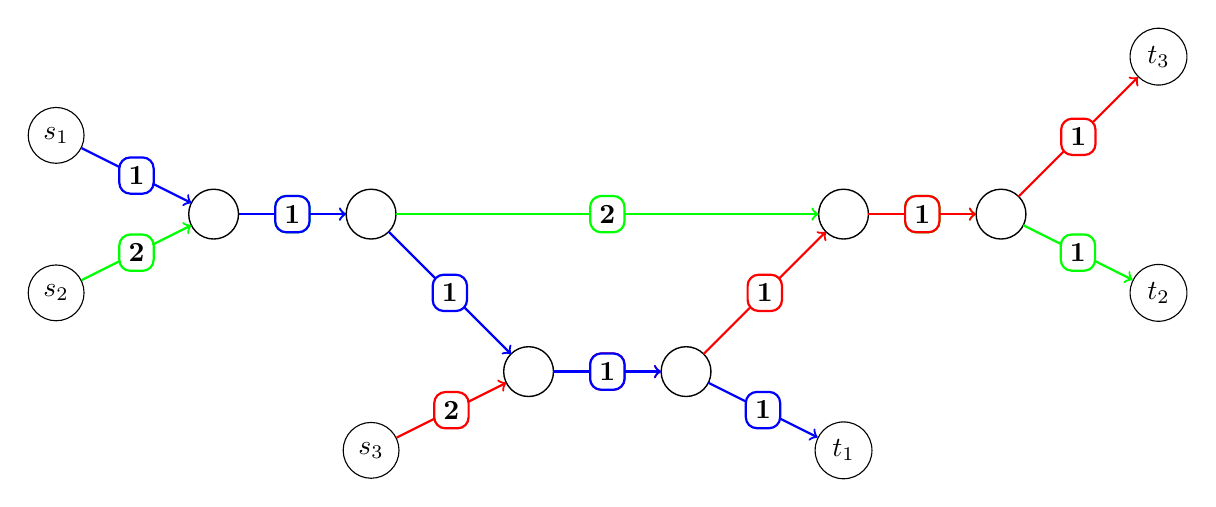
\begin{tikzpicture}


\tikzset{
  LabelStyle/.style = { rectangle, rounded corners, draw,
                       font = \bfseries },
  EdgeStyle/.append style = {->} }
  \SetGraphUnit{5}
  \node[draw,circle] (s3) at (4, 2) {$s_3$}; 
  \node[draw,circle] (s2) at (0, 4) {$s_2$}; 
  \node[draw,circle] (s1) at (0, 6) {$s_1$}; 

  \node[draw,circle] (t3) at (14, 7) {$t_3$}; 
  \node[draw,circle] (t2) at (14, 4) {$t_2$}; 
  \node[draw,circle] (t1) at (10, 2) {$t_1$}; 

  
  \SetVertexNoLabel
  \Vertex[x=2,y=5]{A}
  \Vertex[x=4,y=5]{B}
  \Vertex[x=10,y=5]{C}
  \Vertex[x=12,y=5]{D}
  \Vertex[x=6,y=3]{E}
  \Vertex[x=8,y=3]{F}
  \tikzset{
  EdgeStyle/.append style = {green} }
  \Edge[label = 2](s2)(A)
  \Edge[label = 1](A)(B)
  \Edge[label = 2](B)(C)
  \Edge[label = 1](C)(D)
  \Edge[label = 1](D)(t2)

  
   \tikzset{
  EdgeStyle/.append style = {red} }
  \Edge[label = 2](s3)(E)
  \Edge[label = 1](E)(F)
  \Edge[label = 1](F)(C)
  \Edge[label = 1](C)(D)
  \Edge[label = 1](D)(t3) 
     \tikzset{
  EdgeStyle/.append style = {blue} }
  \Edge[label = 1](s1)(A)
  \Edge[label = 1](A)(B)
  \Edge[label = 1](B)(E)
  \Edge[label = 1](E)(F)
  \Edge[label = 1](F)(t1)

\end{tikzpicture}

}
     \end{center}
       \caption{A routed network with $(0,0,0)$ as a $(2,1)$-periodic assignment}
       \label{fig:example}
      \end{figure}


   \subsection{Problems}\label{nonmonotone}

    We want to find an assignment which allows to send periodic messages from sources to targets
    without collisions. We introduce the following associated decision problem, useful for hardness proofs.
    

      \noindent {\bf  Periodic Routes Assignment (PRA)} 

      \noindent {\bf Input:} a routed network $(G,\cal R)$, an integer $\tau$ and an integer $P$.

      \noindent {\bf Question:} does there exist a $(P,\tau)$-periodic assignment of $(G,\cal R)$ ?


      We will prove in Sec.~\ref{sec:complexity} that the problem PRA is $\NP$-complete, even in restricted settings.
      Even approximating the smallest value of $P$ for which there is a $(P,\tau)$-periodic assignment is hard.
      
      An unusual property of assignment is that given a routed network, we may have a $(P,\tau)$-periodic assignment but no
      $(P',\tau)$-periodic assignment with $P' > P$: the existence of an assignment is not monotone with regards to $P$.

	\begin{lemma} \label{lemma:monotonic}
	 For any odd $P$, there is a routed network such that there is $(2,1)$-periodic assignment but no $(P,1)$-periodic assignment.
	\end{lemma}
\begin{proof}

      Consider the routed network $(G,{\cal R})$ given in the previous subsection. 
      We change the weights so that for $v$, the first vertex which belongs to $r_i$ and $r_j$,
      we have $\lambda(v,r_i) - \lambda(v,r_j)= P$, where $P$ is an odd number smaller than $n$, the number of routes in ${\cal R_{\cal C}}$. In such a graph, there is no $(P,\tau)$-periodic assignment, since the problem reduces to finding a $P$-coloring in a complete graph with $n > P$ vertices, the colors beings the offsets of the routes.\\
      If we consider a period of $2$, for all $i \neq j$, $\lambda(v,r_i) - \lambda(v,r_j) \mod 2 = 1$ . Therefore $(0,\dots,0)$ is a $(2,1)$-periodic assignment of ${\cal R}$.

      
\end{proof}
      
      In the context of cloud-RAN applications, we need to send message from a RRH $u$ to a BBU $v$ and then 
      we must send the answer from $v$ back to $u$. We say that a routed network $(G, {\cal R})$ is \textbf{symmetric}
      if there is a bijection $\rho$ between routes such that for any route $r$ with first vertex $u$ and last vertex $v$, $\rho(r)$ has first vertex $v$ and last vertex $u$. In all practical cases the routes $r$ and $\rho(r)$ will be the same with the orientation of the arcs reversed, which corresponds to bidirectional links in the networks, but we need not to enforce this property.

         
         We now give a new interpretation of a $(P,\tau)$-periodic assignment of a $(G,{\cal R})$ symmetric routed network, so that it represents the sending of a message and of its answer.
	This assignment represents the following process: first a message is sent at $u$, through the route $r$, at time $m$.
       
      
      
      \begin{center}
      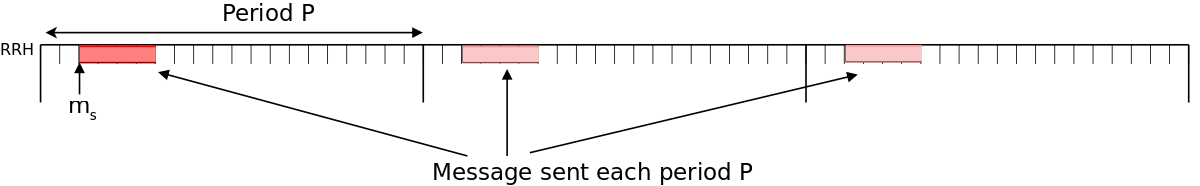
\includegraphics[scale=0.3]{rrh.png}
      \end{center}
      
      

      This message is received by $v$ the last vertex of $r$ at time $t(v,r)$. It is then sent back to $u$ on the route $\rho(r)$ in the same period at time $m_{\rho(s)}$ if $m_{\rho(s)} > t(\rho(s),r)$, otherwise at time $m_{\rho(s)}$ in the next period. The time between the arrival of the message and the time it is sent back is called the \textbf{waiting time} and is defined by $w_s = m_{\rho(s)} - t(\rho(s),r)$ if $m_{\rho(s)} > t(\rho(s),r)$ and $w_s = m_{\rho(s)} + P - t(\rho(s),r)$ otherwise.
 
       \begin{center}
      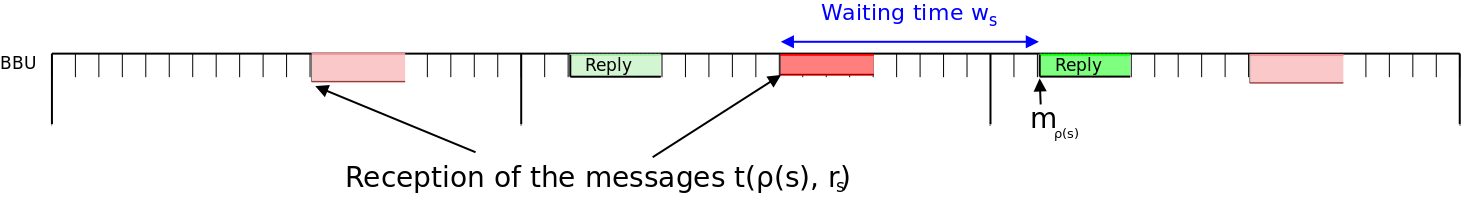
\includegraphics[scale=0.17]{BBU2.png}
      \end{center}
     

      When a BBU receives a message, it must compute the answer before sending it back to the RRH. This time can be encoded
      in the last arc leading to the BBU and thus we need not to consider it explicitly in our model.
    
      Thus, the whole process time for a message sent at vertex $s$ on the route $r$ is equal to
      $$
      PT(s)=\lambda(r)+ w_s+\lambda(r).
      $$
      
      In the process time, we count the time between the first time at which a message is emitted and 
      the first time at which the message comes back. Alternatively we could consider the time between the emission of the first slot and the reception of the last slot of the message, which would add $\tau$ to the process time.
      However, since all messages are of size $\tau$, it will not change the problem we solve in the rest of the article and that we now introduce.
      
    The {\bf maximum process time} of the $(P,\tau)$-periodic assignment ${\cal M} $ is defined by $MT({\cal M})=\max\limits_{s \in S} PT(s)$. We consider the following decision problem.

      \noindent {\bf Periodic Assignment for Low Latency (PALL)} 

      \noindent {\bf Input:}  A symmetric routed network $(G,{\cal R})$, a period $P$, an integer $\tau$, an integer $T_{max}$.

      \noindent {\bf Question:} does there exist a $(P,\tau)$-periodic assignment ${\cal M}$ of $(G,{\cal R})$ such that $MT({\cal M}) \leq T_{max}$?

      As a consequence of the $\NP$-hardness of PRA, we show in the next subsection that this problem is $\NP$-hard. 
      In Sec.~\ref{sec:PALL} we will study heuristics which try to solve the search version of PALL (computing an assignment), also denoted by PALL for simplicity.

  
\section{Hardness of PRA}
  \label{sec:complexity}

 In this section we always assume that the size of a message $\tau$ is equal to one. 
 We will prove the hardness of PRA and PALL for $\tau =1$ which implies the hardness of the general problems. 
Consider an instance of the problem PRA, i.e., a routed network $(G,\cal{R})$ and a period $P$.
The {\bf conflict depth} of a route is the number of other routes which share an edge with it. 
The conflict depth of a routed network $(G,\cal{R})$ is the maximum of the conflict depth of the routes in $\cal{R}$.
The {\bf load} of a routed network is the maximal number of routes sharing the same arc.
Remark that a $(P,1)$-periodic assignment must satisfy that $P$ is larger or equal to the load.


We give two alternate proofs that PRA is $\NP$-complete.
The first proof works already for conflict depth two. Remark that for conflict depth one,
the graph can be seen as a set of disjoint pair of routes, on which PRA and PALL can be solved in linear time. 
 The second proof reduces the problem to graph coloring and implies inapproximability when one tries to find the smallest possible $P$. \\

 \begin{proposition}
Problem PRA is $\NP$-complete, when the routing is of conflict depth two.
\end{proposition}
 \begin{proof}
 The problem $PRA$ is in $\NP$ since given an offset for each route in an assignment, it is easy to check in linear time in the number of edges whether there are collisions.
 
  Let $H=(V,E)$ be a graph and let $d$ be its maximal degree. We consider the problem to determine whether $H$ is edge-colorable
  with $d$ or $d+1$ colors. The edge coloring problem is $\NP$-hard~\cite{holyer1981np} and we reduce it to PRA to prove its $\NP$-hardness. We define from $H$ an instance of PRA as follows. 
  For each $v$ in $V$, the graph $G$ has two vertices $v_1, v_2$, and for each $(u,v) \in E$,the graph G has two vertices $s_{u,v}, t_{u,v}$. Set an arbitrary orientation of the edge $(u,v)$, such that the following route is directed from $u$ to $v$.
%   The set $A$ of arcs of $G$ is: 
%   $$ \{(v_1,v_2) \mid v\in V\} \cup \{(u_2,v_1)\mid u \neq v \in V^2\} \cup \{(s_{u,v},u_1),(v_2,t_{u,v}) \mid (u,v) \in E \}. $$
  For each edge $(u,v) \in E$, there is a route $s_{u,v},u_1,u_2,v_1,v_2,t_{u,v}$ in ${\cal R}$.  
  All these arcs are of weight $0$. The set of arcs of G is the union between all the arcs of the previous routes.
   
    
  Observe that the existence of a $d$-coloring of $H$ is equivalent to the existence of a $(d,1)$-periodic assignment
  of $(G,{\cal R})$. Indeed, a $d$-coloring of $H$ can be seen as a labeling of its edges by the integers
  in $\{0,\dots,d-1\}$ and we have a bijection between $d$-colorings of $H$ and offsets of the routes of ${\cal R}$.
  By construction, the constraint of having no collision between the routes is equivalent to the fact that no two adjacent edges have the same color. Therefore we have reduced edge coloring to PRA which concludes the proof. 
 \end{proof}
 
 Remark that we have used zero weight in the proof. If we ask the weights to be strictly positive, which makes sense in our model since
they represent the latency of physical links, it is easy to adapt the proof. We just have to set them so that in any route the weight at $u_1$ is equal to $d$ and thus equal to $0$ modulo $d$. We now lift this hardness result to the problem PALL.

\begin{corollary}
Problem PALL is $\NP$-complete for routing of conflict depth two.
\end{corollary}
\begin{proof}
 We consider $((G,{\cal R}),P,\tau)$ an instance of $PRA$. We assume that no vertex is the first of some route and the last of another one. Remark that this condition is satisfied in the previous proof, which makes the problem $PRA$ restricted to this kind of instance $\NP$-complete. 
 Let us define $T_{max} = 2 \times \max_{r \in {\cal R}} \lambda(r) + P$. We define $(G',{\cal R}')$ a symmetric routed network from $(G,{\cal R})$ where for every route we add a symmetric route with new arcs of opposite orientation and the same weights.
 The instance $((G',{\cal R'}),P,\tau,T_{max})$ is in PALL if and only if $((G,{\cal R}),P,\tau)$ is in $PRA$. Indeed the waiting time of each route is by definition less than $P$ and thus the maximal process time is always less than $T_{max}$. Moreover a $(P,\tau)$-assignment of $(G,{\cal R})$ can be extended into a $(P,\tau)$-assignment of $(G',{\cal R'})$ in the following way. For each route $r \in \cal{R}$ starting at $s$, the time at which the message arrives is $t(\rho(s),r)$, then we choose as offset for $\rho(r) \in \cal{R}'$ $-t(\rho(s),r) \mod P$. The symmetry ensures that each new route $\rho(r)$ in ${\cal R'}$ uses the same times slot as $r$ one each of its node and thus avoid collisions.
\end{proof}

Let MIN-PRA be the problem, given a routed network and an assignment, to find the minimal period $P$ such that there is a $P$-periodic assignment. 

\begin{theorem}\label{th:inapprox}
 The problem MIN-PRA cannot be approximated in polynomial time within a factor $n^{1-o(1)}$, with $n$ the number of routes, unless $\P = \NP$ even when the load is two.
\end{theorem}

\begin{proof}
 We reduce graph coloring to PRA. Let $H$ be a graph instance of the $k$-coloring problem. 
 We define ${\cal R}$ in the following way: for each vertex $v$ in $H$, there is a route $r_v$ in ${\cal R}$.
 Two routes $r_v$ and $r_u$ share an arc if and only if $(u,v)$ is an edge in $H$; this arc is the only one shared by these two routes. All arcs are of weight $0$. 
 
 Observe that the existence of a $k$-coloring of $H$ is equivalent to the existence of a $(k,1)$-periodic assignment in $G$, 
 by converting an offset of a route into a color of a vertex and reciprocally. Therefore if we can approximate the minimum value of $P$ within some factor, we could approximate the minimal number of colors needed to color a graph within the same factor. The proof follows from the hardness of approximability of finding a minimal coloring~\cite{zuckerman2006linear}.
\end{proof}


In particular, this reduction shows that even with small maximal load, the minimal period can be large.

    \begin{figure}[ht]
    
    \scalebox{0.5}{
    \begin{tikzpicture}
    \tikzset{
      LabelStyle/.style = { rectangle, rounded corners, draw,
			  font = \bfseries },
      EdgeStyle/.append style = {->} }
      \SetGraphUnit{5}
      
      
      \node[draw,circle] (s3) at (4, 2) {$s_2$}; 
      \node[draw,circle] (s2) at (0, 4) {$s_1$}; 
      \node[draw,circle] (s1) at (0, 6) {$s_0$}; 

      \node[draw,circle] (t3) at (12, 3) {$t_2$}; 
      \node[draw,circle] (t2) at (14, 4) {$t_1$}; 
      \node[draw,circle] (t1) at (10, 2) {$t_0$}; 
      

      \tikzstyle{VertexStyle}=[shape = circle, draw, minimum size = 20pt]
	\tikzset{
      VertexStyle/.append style = {blue} }
	\Vertex[x=-8,y=3]{1}
	      \tikzset{
      VertexStyle/.append style = {green} }
	  \Vertex[x=-7,y=5]{2}

	    \tikzset{
      VertexStyle/.append style = {red} }
	  \Vertex[x=-6,y=4]{3}
		\tikzset{
      VertexStyle/.append style = {black} }
      
      
      \SetVertexNoLabel
      \Vertex[x=2,y=5]{A}
      \Vertex[x=4,y=5]{B}
      \Vertex[x=10,y=5]{C}
      \Vertex[x=12,y=5]{D}
      \Vertex[x=6,y=3]{E}
      \Vertex[x=8,y=3]{F}
      \tikzset{
      EdgeStyle/.append style = {green} }
      \Edge(s2)(A)
      \Edge(A)(B)
      \Edge(B)(C)
      \Edge(C)(D)
      \Edge(D)(t2)

      
      \tikzset{
      EdgeStyle/.append style = {red} }
      \Edge(s3)(E)
      \Edge(E)(F)
      \Edge(F)(t3) 
	\tikzset{
      EdgeStyle/.append style = {blue} }
      \Edge(s1)(A)
      \Edge(A)(B)
      \Edge(B)(E)
      \Edge(E)(F)
      \Edge(F)(t1)
      
	\tikzset{
      EdgeStyle/.append style = {black,-} }

      \Edge(1)(2)
      \Edge(1)(3)
    \node (1) at (-3,4){\Huge $\rightarrow$};
%     
%     \node (2) at (-7,0){\Huge H};
%     \node (3) at (10,0){\Huge G};
    \end{tikzpicture}
    }
    \caption{Reduction from k-coloring to MIN-PRA}

    \end{figure}
    
\section{The star topology: no waiting time} \label{sec:PAZL}
  
   
    
    \subsection{The star topology}
    
      From now on, we will only consider graphs with a very simple topology that we call the {\bf star topology}. 
      First, for each arc $(u,v)$, there is also an arc $(v,u)$ with the same weight.
      There are two sets of vertices, $S=\{s_1,...,s_n\}$ and $T=\{t_1,...,t_n\}$ of cardinality $n$ and two special nodes
      the central source node {\bf $c_s$} and the central target node {\bf $c_t$}. There is an arc between {\bf $c_s$} and {\bf $c_t$} shared by all routes. For all $i$, there is an arc between $s_i$ and $c_s$ and between $t_i$ and $c_t$.
      The routes are the directed paths $r_i = s_i,c_s,c_t,t_i$ and $\rho(r_i) = t_i,c_t,c_s,s_i$ which defines a 
      symmetric routed network. 
      
      
       \begin{center}
	 \scalebox{0.7}{
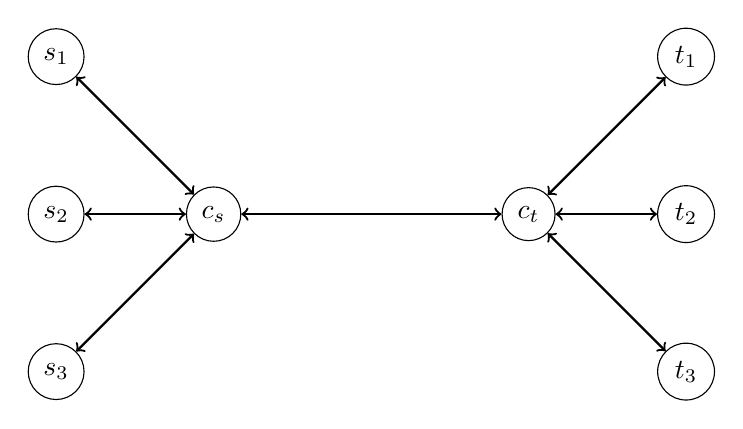
\begin{tikzpicture}

\tikzset{
  LabelStyle/.style = { rectangle, rounded corners, draw,
                       font = \bfseries },
  EdgeStyle/.append style = {<->} }

  \SetGraphUnit{5}
  
  \node[draw,circle] (s3) at (0, 0) {$s_3$}; 
  \node[draw,circle] (s2) at (0, 2) {$s_2$}; 
  \node[draw,circle] (s1) at (0, 4) {$s_1$}; 

  \node[draw,circle] (t3) at (8, 0) {$t_3$}; 
  \node[draw,circle] (t2) at (8, 2) {$t_2$}; 
  \node[draw,circle] (t1) at (8, 4) {$t_1$}; 
  

  \node[draw,circle] (cs) at (2, 2) {$c_s$}; 
  \node[draw,circle] (ct) at (6, 2) {$c_t$}; 

  
  \Edge(s1)(cs)
  \Edge(s2)(cs)
  \Edge(s3)(cs)
  
  \Edge(ct)(t1)
  \Edge(ct)(t2)
  \Edge(ct)(t3)
  
  \Edge(cs)(ct)

  
\end{tikzpicture}
}

  \end{center}
	
      Since the central arc appears in every route, its value do not matter when considering the process time of an assignment.
      Moreover an assignment without collisions is also an assignment without collisions if the weight of the central arc 
      is set to $0$, therefore we assume from now on it is indeed $0$.
      Collisions between messages can only appear in the arcs after node $c_s$ on the way forward and after node $c_t$ on the way back.
      Thus, we only have to check if there is no collisions in a given period at those two vertices.
      We try to order the messages such that they can pass thought the common arcs in a time window of $P$ max. We define the {\bf forward period}, a time window of size P at the beginning of the arc after $c_s$, and the {\bf backward period} the one at the beginning of the arc after $c_t$. A message issued on the route $r$ at time $m_s$ will reach $c_s$ at time $m_{s} + t(c_s,r) \mod P$ in the forward period. If the offset of $\rho(s)$ is $m_{\rho(s)}$, the answer will reach $c_t$ at time $m_{\rho(s)} + t(c_t,\rho(r))\mod P$ in the backward period.

      A $(P,\tau)$-periodic assignment is then a choice for all $i < n$, of $m_{r_i}$ and $m_{\rho(r_i)}$ such that, for any couple $(i\neq j)$, we have $[t(c_s,r_{i})] \cap [t(c_s,r_{j})] = \emptyset$ and $[t(c_t,\rho(r_i))] \cap [t(c_t,\rho(r_j))] = \emptyset$.

      

  \subsection{Solving PAZL}
  
  In this subsection, we deal with a simpler version of the problem PALL.
  We ask for a $(P,\tau)$-periodic assignment {\bf with all waiting times equal to $0$} and we call this restricted problem {\bf Periodic Assignment for Zero Latency} or PAZL. 
  In that case $MT({\cal M})$ is equal to twice the weight of the longest route, thus $T_{max}$ is not relevant anymore. 
  Since $w_i=0$, choosing $m_{s_i}$, the offset of the route from $s_i$ to $t_i$, also sets the offset of the route from $t_i$ to $s_i$ to $m_{s_i} + \lambda(r_i) \mod P$.
  Remark that there is a bijection between the assignments of a star topology and the 
  assignments of the same star topology where all arcs from $s_i$ to $c_s$ have weight equal to $0$ by changing $m_{s_i}$ into $m_{s_i} - t(c_s,r_i) \mod P$. Therefore we assume from now on that the \emph{weight of the arcs from $s_i$ to $c_s$ are all equal to $0$}.
  
  We propose two algorithms that always find a solution in polynomial time if instances meets some criteria (short routes or great enough period) but which may fail in other cases and one exponential algorithm which always finds a solution if it exists.
  
    \subsubsection*{Shortest-longest policy}
    

    We first present a simple policy, which works when the period is large with regards to the weight of the routes.
    The messages are sent in order from the shortest route to the longest route, without any gap between two messages in the forward period.
    In other words, we assume that the route $r_i$ are sorted by increasing $\lambda(r_i)$ and we set $m_{s_i}$ the offset of $r_i$ to $(i-1)\tau$. We call this algorithm {\bf Shortest-Longest}.
      
     By definition, there are no collision in the forward period and if the period is long enough, 
     it is easy to see that in the backward period the order of the messages are the same as in the forward period and that no collision can occur. 
      
      
      \begin{proposition} When $n\tau + 2(\lambda(r_{n}) - \lambda(r_{1})) \leq P$,
      there is always a solution to PAZL and Shortest-Longest finds it  in time $O(n\log(n))$.\label{prop:SL}
      \end{proposition}
      \begin{proof}
       Since $m_{s_i} = (i-1)\tau$, $[t(c_s,r_{i})] = \{i\tau,\dots, (i+1)\tau -1\}$ and there are no collision on the forward period.
       
       
       We may assume that $\lambda(r_{1}) = 0$, since removing $\lambda(r_{1})$ from every arc $(c_t,t_i)$ does not change the order on the length of the routes nor the collisions between messages.
       Since $\lambda(r_{1}) = 0$, by hypothesis we have $n\tau + 2\lambda(r_{n}) \leq P$ which implies that
       $[t(c_s,r_{i})] = \{2 \lambda(r_{i}) + (i-1)\tau, \dots,  2 \lambda(r_{i}) + i\tau -1\}$.
       Since $ \lambda(r_{i}) \leq  \lambda(r_{i+1})$ by construction, we have  $2 \lambda(r_{i}) + i\tau -1 < 2 \lambda(r_{i+1}) + i\tau$ which proves that there are no collision on the backward period. 
       
       The complexity of the algorithm is dominated by the sorting of the routes in $O(n\log(n))$. 
      \end{proof}

      If the period is slightly smaller that the bound of Proposition~\ref{prop:SL}, a collision will occur on the first route in the backward period. Hence, this policy is not useful even as a heuristic for longer routes as confirmed by the experimental results of Subsection~\ref{sec:exp_PAZL}. 

   
    \subsubsection*{Greedy Algorithm}
    
    We propose a greedy algorithm to build a $(P,\tau)$-periodic assignment, which provably works when
    the period is large enough with regards to the number of routes and size of messages. In other words, 
    we can always find a solution when the network is far from saturated. This algorithm defines an upper bound for the period. As a reminder, the lower bound is $n\tau$, that is, the size taken by the messages to be emitted.
    
    \begin{proposition}
    Let  $n$ be the number of routes and let $ 3n\tau \leq P$, then there is is always a solution to PAZL and there is an  algorithm which finds the assignment in time $O(n^2)$.
    \end{proposition}
    \begin{proof}
     We consider the forward period and cut it into consecutive interval of size $\tau$ that we call macro-slots. The algorithm works by choosing an offset for each route in the following way: try all offsets which put the message in a yet not used macro-slot in the forward
     period. The choice of an offset also fixes the position of the message in the backward period, chose the first one which does not create a collision. We now prove that this algorithm always finds a $(P,\tau)$-periodic assignment without waiting time when $P \geq 3n\tau$.
     
     Assume we are choosing the offset of the route $r_{k+1}$, we have at least $P - k \geq 3n - k$ free macro-slots in the forward period, since $P \geq 3n\tau$. Each of these $3n - k$ possible offset values translates into $3n - k$ positions of messages in the backward period. All these positions are separated by at least $\tau$ slots. There are already $k$ messages of size $\tau$ in the backward period. One such message can intersect at most $2$ potential positions since they are disjoint intervals. Therefore  amongst the possible $3n - k$ positions, there are  at least $3n - k -2k$ which are without collision. Since $k < n$, $3n - k -2k \geq 1$, which proves that the algorithm terminates and find a  $(P,\tau)$-periodic assignment. 
     
     This algorithm works with a complexity $O(n^2)$, since for the $k^{\text{th}}$ route we have to try at most $2k$ offsets before finding a correct one. We can test the $2k$ offsets of the backward period in time $O(k)$ by maintaining an ordered list of the intervals used by already set routes.
     \end{proof}
     
      \begin{center}
      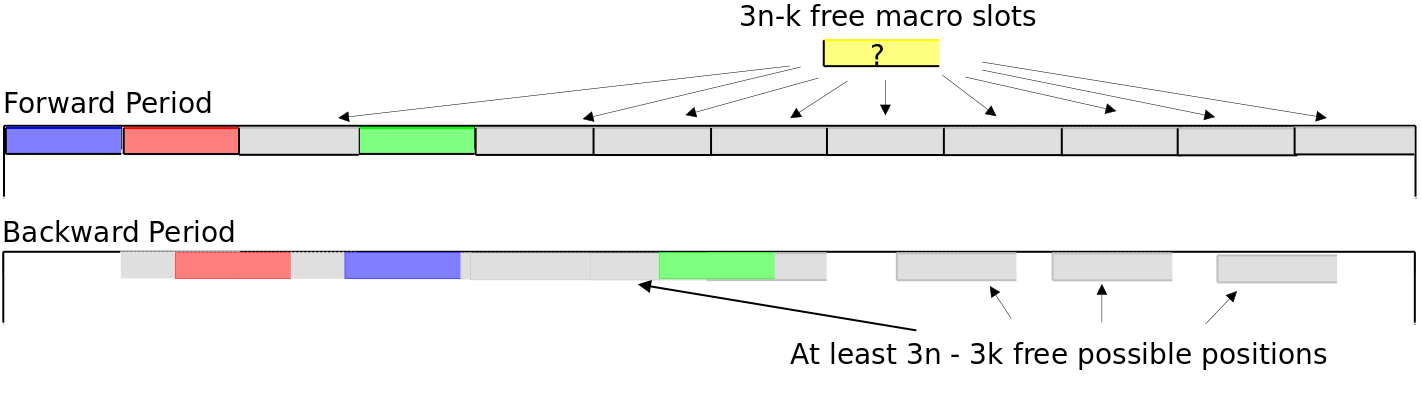
\includegraphics[scale=0.3]{ex3nt.png}
      \end{center}
% 	\begin{algorithm}[H]
% 	\caption{Greedy assignment}
% 	\begin{algorithmic}
% 	\REQUIRE ${\cal R}_{\cal C}$, period $P$
% 	\ENSURE A P-periodic assignment in p $\leq P$, or FAILURE
% 	\STATE $T$ a table of the macro slots of size $\tau$ in the forward period.
% 	\STATE $L$ a list of free intervals in the backward period%$P2[P]$ slots backward period.
% 	\FORALL{source $s$ in S}
% 
% 	\FORALL{free intervals $[a,b]$ in $L$}
% 	\FORALL{ $a/\tau - \lambda(s) <j< b/\tau - \lambda(s)$ }
% 	\IF{ $T[j] == FREE$}
% 	\STATE $m_{s} \leftarrow j.\tau$
% 	\STATE $T[j] = USED$
% 	\STATE update $[a,b]$ in $L$
% 	\STATE BREAK
% 	\ENDIF
% 	\ENDFOR
% 	\ENDFOR
% % 	
% % 	\IF{No intervals are found for $s_i$}
% % 	\STATE return FAILURE
% % 	\ENDIF
% % 	\ENDFOR
% 
% 	\ENDFOR
% 
% 	\end{algorithmic}
% 	\end{algorithm}
	
This algorithm, contrarily to the previous one, may work well, even when the condition $P \geq 3n\tau$ is not true.
In fact, experimental data in Subsection~\ref{sec:exp_PAZL} suggests that the algorithm finds a solution on average when $P \geq 2 n\tau$.
Note that we also experimented with other greedy algorithms which do not use macro-slots, they work even better in practice but their theoretical upper bound is worse.

	\subsubsection*{Exhaustive search}
% 	\begin{algorithm}[H]
% 	\caption{Exhaustive Generation}  
% 	\begin{algorithmic}
% 	\REQUIRE A routage graph ${\cal R}_{\cal C}$, period $P$, packet size $\tau$
% 	\ENSURE $(P,\tau)$-periodic assignment of ${\cal R}_{\cal C}$
% 	\STATE Forward-budget $\leftarrow$ $P$ - n * $\tau$
% 	\STATE Backward-budget $\leftarrow$ $P$ - n * $\tau$
% 	\STATE Free-Intervals $\leftarrow$ list of free intervals in the backward period, init to $[0;P[$
% 	\FORALL{source $s_i$ in S}
% 	\FORALL{j in Free-Intervals }
% 	\IF{Message of the route $r_{s_i}$ does not collides with scheduled routes}
% 	\STATE $m_{s_i} \leftarrow $ the first slot of Free-Intervals[j]
% 	\STATE Split the Free-Intervals considering the new packet
% 	\STATE Forward-budget $\leftarrow$ Forward-budget - {\em lost size}
% 	\STATE Backward-budget $\leftarrow$ Backward-budget - {\em lost size}
% 	\STATE call Exhaustive Generation on remaining routes
% 	\ENDIF
% 	\ENDFOR
% 	\ENDFOR
% 
% 
%       \end{algorithmic}
%       \end{algorithm}

% 	    
      We now present an exhaustive search algorithm, which tries to set the offsets in all possible ways until it has found a $(P,\tau)$-periodic assignment. Contrarily to the two previous algorithms, when it fails to find a solution, then it certifies there are no solution to PAZL.
      
      We have $n$ routes denoted by $\{0,\dots,n-1\}$. A partial solution $S$ is 
      a partial function from $[n]$ to $\{0,1,\dots,P-\tau -1\}$ which sets a starting time for a subset of the routes $R(S) \subseteq [n]$, such that there are no collisions for these routes.  A partial solution $S'$ extends $S$, if $S'$ is defined over one more route than $S$ and this route has a larger starting offset than all routes of $S$: $R(S') = R(S) \cup \{r'\}$ and for all  $r \in R(S)$, $S(r) + \tau \leq S'{r'}$. We define a tree whose nodes are partial solutions and such that the root is the empty partial solution and 
      the children of a partial solution are the partial solutions which extend it. The solutions to our problem will be the leaves of depth $n$ in the tree, and our exhaustive search algorithm is a depth-first search of this tree. 
      
      Remark that a node $S$ with $|R(S)| = k$ can have as many as $(n-k)P$ children. Since the tree is of depth $n$, the tree may have as many as $n!P^n$ elements and while $n$ is small, $P$ may be large which makes its traversal intractable.  Therefore we have to find cuts in the tree to avoid to explore it entirely and henceforth make the algorithm practical. Cuts correspond to the detection of subtrees which contain no solutions or solutions which can be found elsewhere and can thus be skipped. We now propose three cuts, the first two being particularly useful when the network is loaded ($n\tau$ is not far from $P$). 
      
      \begin{enumerate}
       \item We consider the number of slots which can be used by routes not yet fixed by a partial solution in the \emph{forward period}. When we extend a solution into $S$ with a new route at offset $m$, then at most $(P - m) / \tau $ routes can still be used to extend $S$ without collisions in the forward period. If that value is less than the number of routes which are not in $R(S)$, it is a failure and the algorithm backtracks.
       
       \item 
       For the next two cuts, we need to define the notion of the useful slots of a partial solution $S$ in the \emph{backward period}: a slot is said to be useful, if it is not used by a message set by $S$ in the backward period and it belongs to an interval of at least $\tau$ such slots. Useful slots are positions of the backward period which can be used when extending $S$. We will denote by $([a_i,b_i[)_{i\leq l}$ the ordered sequence of intervals of useful slots of $S$. Without loss of generality we can assume that all $a_i, b_i \leq l$. The number of messages of size $\tau$ which can be placed in the useful slots of $S$ is thus  $\displaystyle{ \sum_{i=0}^{l} (b_{i} -a_i)/\tau } $. If that value is less than the number of routes which are not in $R(S)$, it is a failure and the algorithm backtracks. Notice that the list of intervals of useful slots and the value $\displaystyle{ \sum_{i=0}^{l} (b_{i} -a_i)/\tau } $ can be maintained in constant time, since each time a route is added, we only need to split an interval of useful slots into at most two such intervals.
       
       
       \item 
       Let $S_1$ and $S_2$ be two partial solutions with $R(S_1) = R(S_2)$. Let $US_1$ (respectively $US_2$) be the set of useful slots of $S_1$ (resp. $S_2$). We say that \emph{$S_1$ dominates $S_2$} if there are more useful slots both in the forward and backward periods for $S_1$ than for $S_2$. Formally, the largest offset fixed in $S_1$ is smaller than the one in $S_2$ and $US_2 \subseteq US_1$. Remark that any valid sequence of extensions of $S_2$ (choosing offsets of routes in the complementary of $R(S_2)$) is also a valid sequence of extensions of $S_1$. Therefore if the tree rooted at $S_2$ contain a solution, then $S_1$ contains one too. Hence, in our exhaustive search of the tree of partial solutions, we can skip the tree rooted at $S_2$.
       
       We now explain how we can detect some partial solutions which are dominated so that we do not explore their subtrees.
       Consider a partial solution $S$ which we extend into $S'$ by setting the offset of the route $r$ to be the smallest possible. The offset of $r$ in the backward period is $S'(r)+ \lambda$ and we denote the end of the message before before by $a$. Hence all extensions of $S$ into $S''$ such that $S'(r)  < S''(r) < a + \tau - \lambda$ are dominated by $S'$. Therefore when computing the extension of $S$, we first build $S'$ and then $S''$ with $S''(r) =  a + \tau - \lambda$ , skipping all values in between.
       
       \end{enumerate}
      
      The third cut works well in conjunction with the first one since it makes the offsets grow quickly and 
      which makes the first cut more likely to apply. A last cut could be implemented: compute for every route not in $R(S)$ the set of possible positions in the backward period and verify whether at least one is contained in the useful slots of $S$.


    \subsection{Experimental Evaluation}\label{sec:exp_PAZL}
      
      The following experimental results compare the three presented algorithms.
      Notice that both Greedy algorithm and Shortest-Longest are polynomial time algorithm but are not always able to find a solution. On the other hand, the exhaustive search will find an optimal solution, if it exists, but works in exponential time. We will compare the performance of the algorithms in two different regimes: routes are either short with regards to $\tau$ and $P$, or unrestricted.
      We choose the following realistic parameters with regard to our C-RAN context. The number of routes 
      is at most $n = 20$, $\tau$ is equal to $2500$ and the period is at most $3n\tau$ (otherwise the greedy algorithm always returns a solution). The code in C is available online on the webpages of the authors ~\cite{webpage}.
%             
%             The graphs 
%       To correspond with the C-RAN applications, we made some simulations on graphs in which $\lambda(c_s,r_{s_i})$ and $\lambda(c_t,r_{t_i})$, are drawn following an uniform act between 0 and 700 slots, that is, at the most, 5 km between the RRH and its BBU. The messages size $\tau$ is to 2500 slots, that is, approximately 1.228 Gbps of data for each route. The size of a slot is given by the time taken to send 64 bytes on the network, in which the links has 10Gbps throughput.
% 
%       \todo{Mettre les données concrètes plus proprement et éventuellement ne pas les mettre si on envoie pas à un truc de télécom}

      \paragraph{Short routes}
      
      First we consider routes which are shorter than $\tau$, that is a message cannot be contained 
      completely in a single edge. This is very common in our context and we will consider graphs in which the values $\lambda(c_t,\rho(r_{i}))$ are drawn uniformly between $0$ and $700$ slots. It corresponds to messages of approximately 1Mb, links of bandwidth 10Gbps and length less than 5km between the BBU and the RRH. 
      
      Our aim is to understand how well the algorithms are working when the network has a high load (when 
      the load is low, the greedy algorithm always returns a solution). To do that we try to evaluate the 
      minimal period for which a $(P,\tau)$ periodic assignment can be found by each algorithm. 
      To that end we use linear search on $P$, since a dichotomy method would not work because of Lemma~\ref{lemma:monotonic}.
      
      In our experiment, we generated $1000$ random instances of PAZL for $1$ to $12$ routes. 
      We measured the average minimal period, for each algorithm. We needed to stop our experiments at $12$ routes since the exhaustive search was taking more than a second to finish on many instances.
      Note that the exhaustive search is optimal, that is it finds the best possible period for a given instance. 
      We also drew the functions $f(n) = n\tau$, which is an absolute lower bound on the period and $g(n) = 3n\tau$ which is the theoretical upper bound of the greedy algorithm.
      
      
        
      \begin{figure}

      \begin{center}
	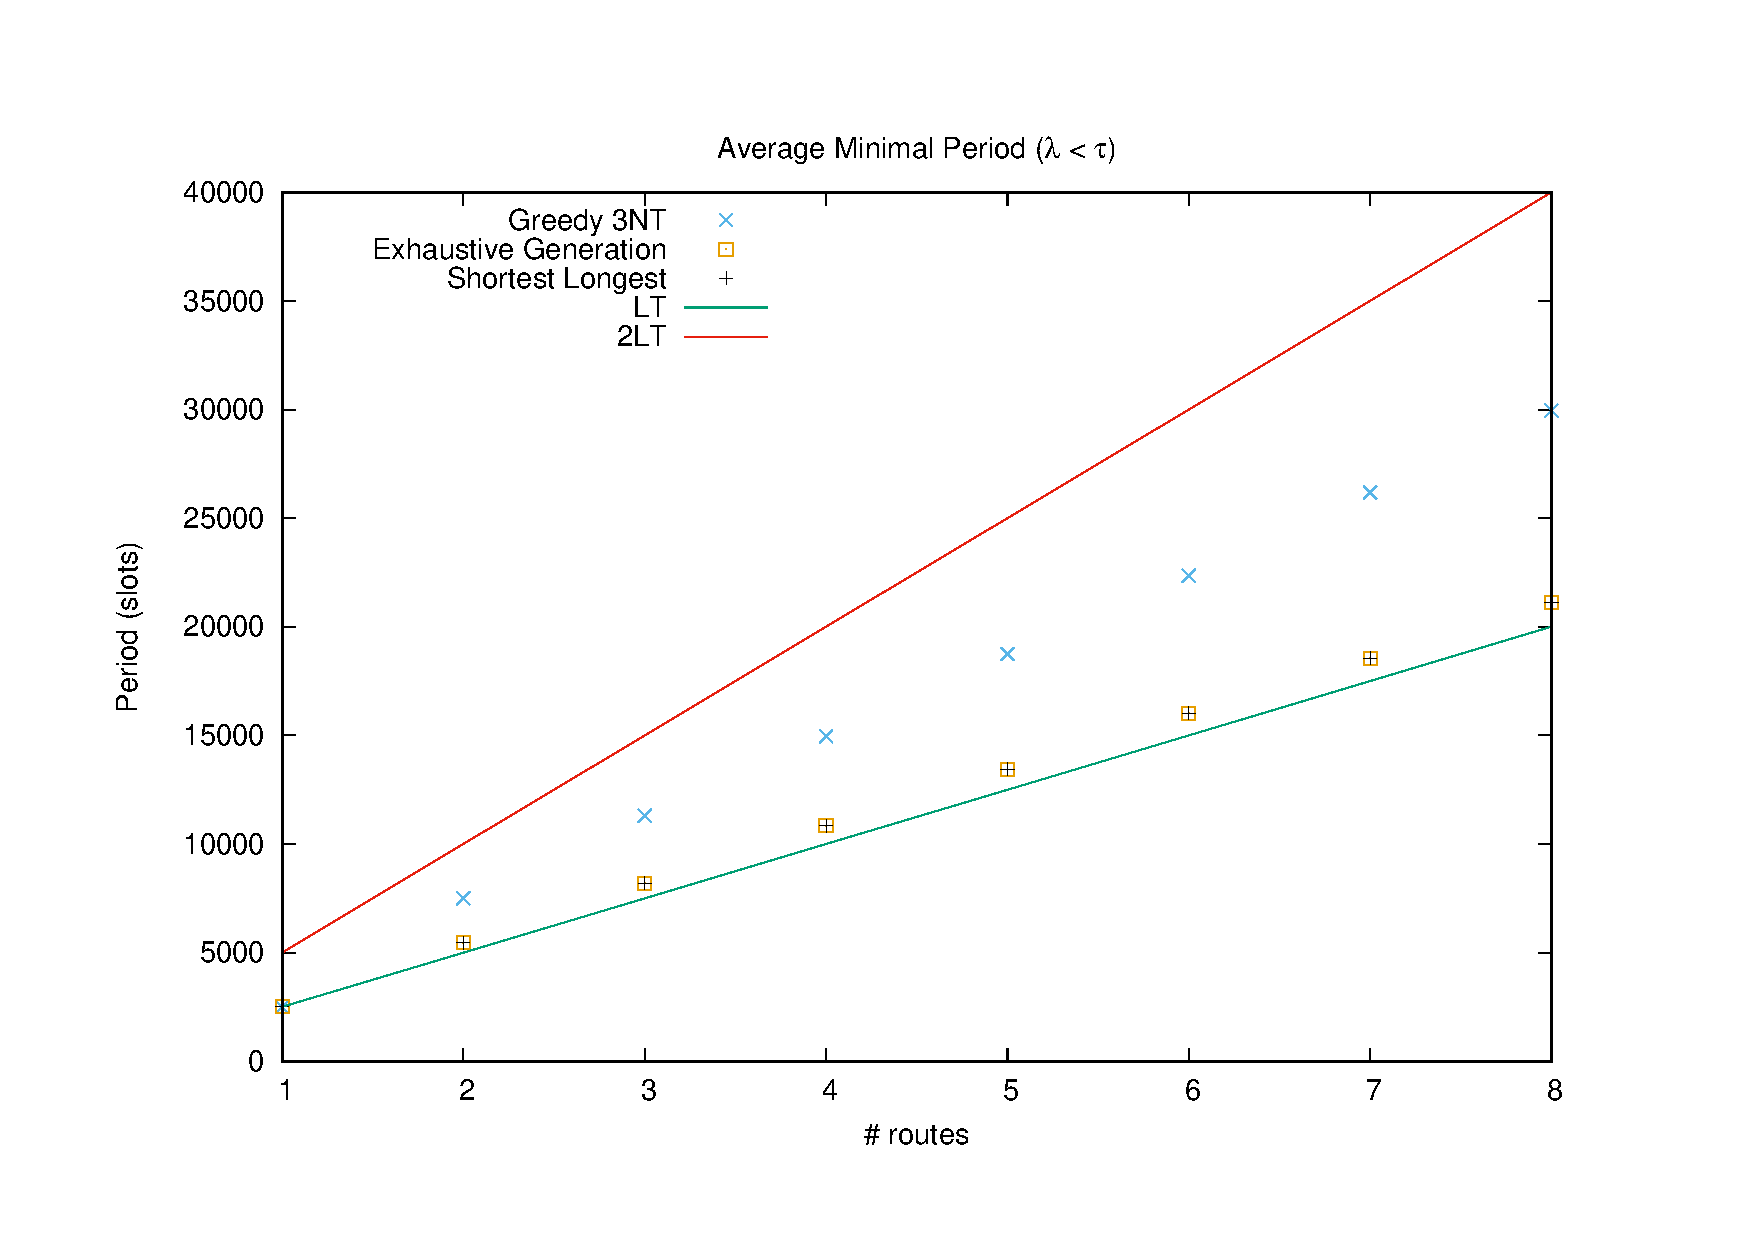
\includegraphics[scale=0.4]{periode_petite.pdf}
      \end{center}
      \caption{Minimum period averaged over $1000$ random instances}
      \end{figure}
      
      First, we remark that the period found by the exhaustive search is only very slightly above the lower bound of 
      $n\tau$, which means that, in this regime, it is very well justified to look for a solution without waiting time even for a highly loaded network. 
      
      The period needed by Shortest-Longest to find an optimal solution is determined by the difference between the longest and the shortest route and could be easily determined theoretically. The algorithm was expected to be good since the routes are short, but it turns out it always finds the optimal solution in our experiments. Therefore, we should use it in practical application, in this regime, instead of the exhaustive search which is much more computationally expensive. 
      
      Finally we remark that the greedy algorithm has an average period much lower than the theoretical upper bound of $3n\tau$. We made a linear regression on this value and with a correlation coefficient greater than $0,999$ we find a slope of $1.53n\tau$.
      
      

      \paragraph{Long routes}
      
      We now want to understand the performance of these algorithms when the size of the routes are unbounded. When the routes are long, the cuts in the exhaustive search are less efficient and thus even for a small number of routes the algorithm may be impractical. To make the experimentations short enough, we have bounded the number of nodes of the tree of partial solutions the exhaustive search can visit by $10^9$.
      
      In this experiment we will fix the number of routes to $8$ and the values $\lambda(c_t,\rho(r_{i}))$ are drawn following an uniform distribution between $0$ and $30000$ slots (in the same range as the period).
      We measure for each algorithm its percentage of success, for periods from $20000$ which is the minimum possible to $50000$.
      
      The exhaustive search can fail because there are no solutions or because it does not have enough time to finish its calculation. Hence we represent both the success rate of the algorithm, and an upper bound on the success rate of any algorithm solving PAZL by combining its successes and its failures because of lack of time. 
      
\begin{figure}

       \begin{center}
      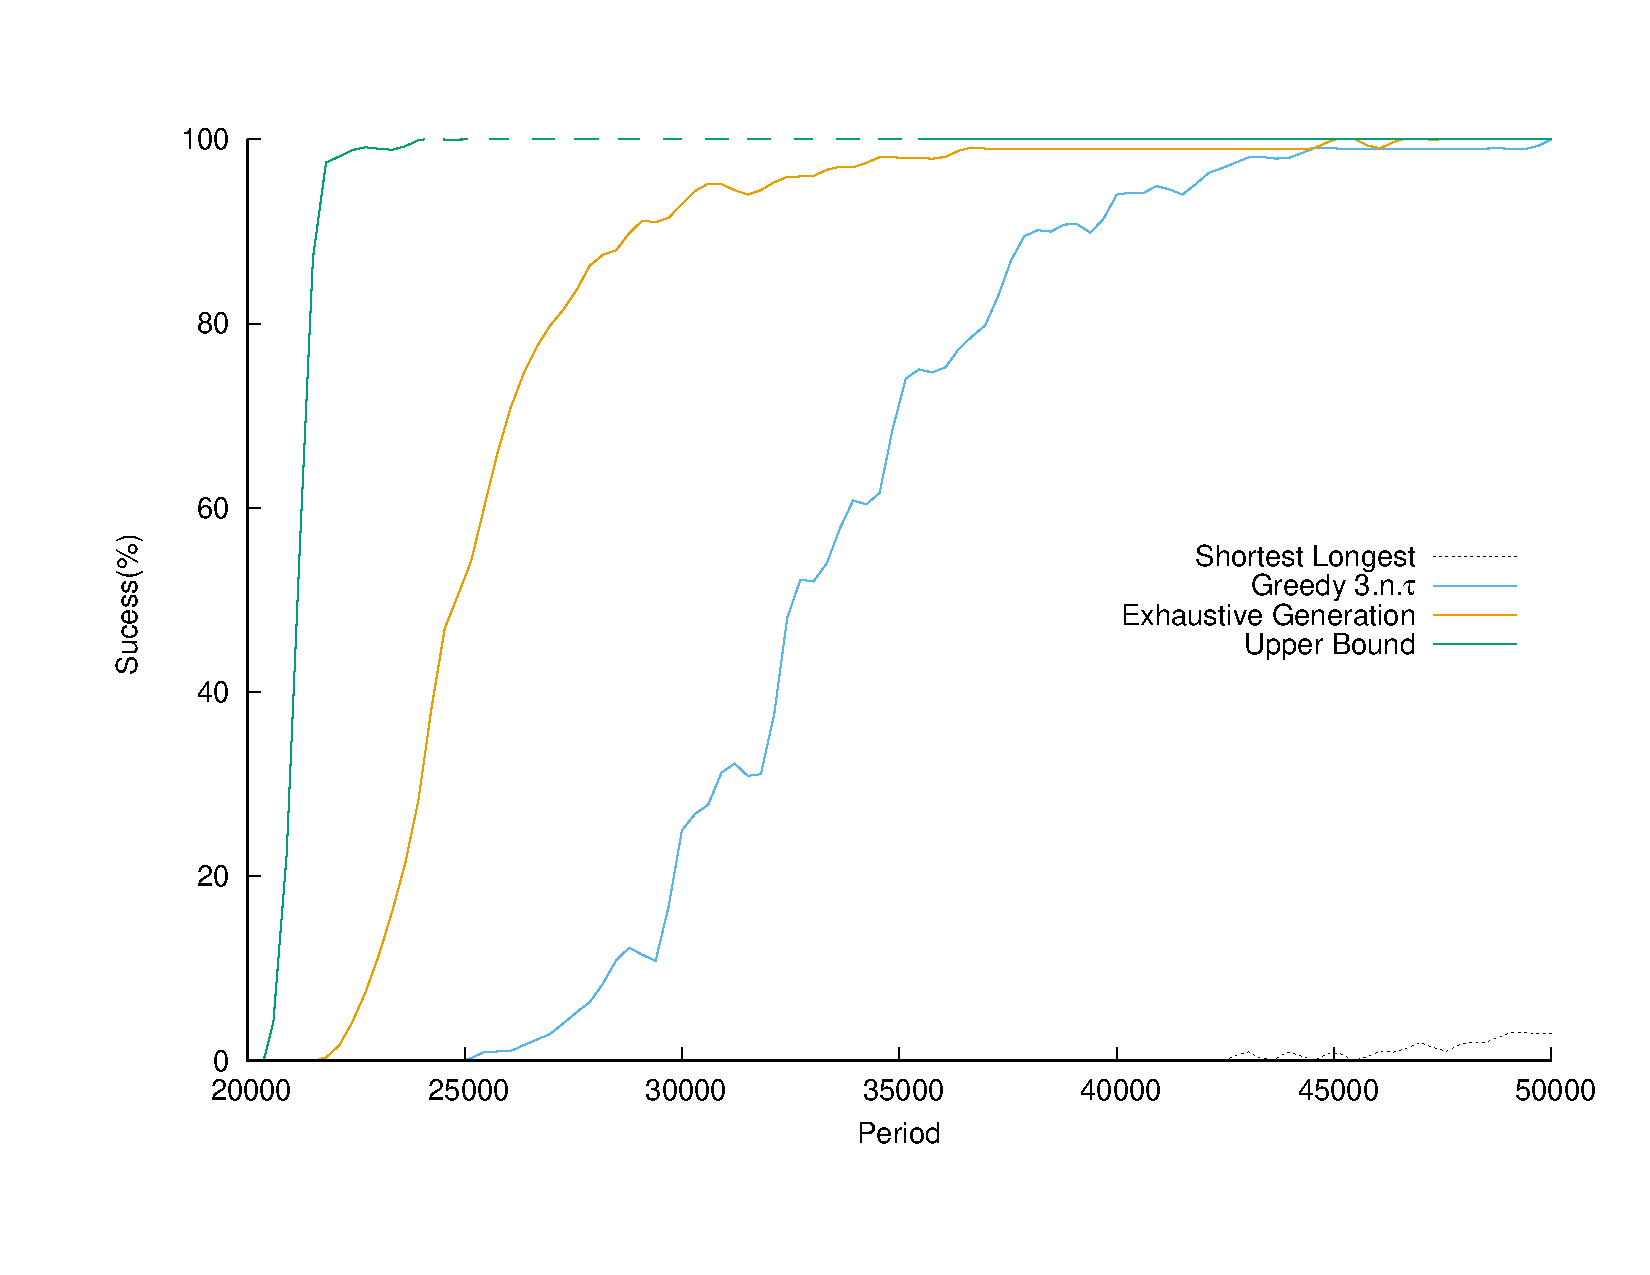
\includegraphics[scale=0.4]{echec_longues.pdf}
      \end{center}
      \caption{Success rate for $8$ routes over $1000$ random instances}
     \end{figure}
      
      In this regime, the performances of Shortest-Longest are abysmal since it depends on the difference between the longest and the smallest route
      which is large here. On the other hand, the greedy algorithm has a performance not so far from the case of short routes, which is expected since it does not directly depend on the size of the route. When repeating the experiments of the previous section on routes of arbitrary length, we find that on average the greedy algorithm finds a solution if $P > 1.89n\tau$.
      
      When the period is less than $40000$, the exhaustive search find many more solutions than the greedy algorithms which justifies its use. 
      However for small period, less than $30000$ the computation time is really important and without improvements it would not be possible to tackle 
      larger problems with $10$ to $20$ routes. Moreover, examining the upper bound curve for small periods less than $22000$, we see that there are very few instances with a solution for PAZL. It means that with long routes and high load, looking for an assignment without waiting time is far too restrictive.
      That is why we present algorithms for the general PALL problem in our next section. We will test them on $8$ long routes and a period between $20000$ and $30000$ where, as we have shown here, there are often no easy to compute assignment without waiting times.
      
   \section{The star topology: minimizing latency}\label{sec:PALL}
    
    In this section, we still work on the start topology, but, from now, we allow the messages to wait in the target vertices (BBU),in order to find some solution that we cannot find with PALL. From now, the process times  $PT$ of the routes can be greater than twice the weight of the routes, but it might not be superior to $T_{max}$.

	\subsection{Particular cases}
		
	One of the closest approach to real networks is the case in which all the weight on the arcs going from $c_t$ to targets are the same and so can be simplified by $0$. In that case, the order of the messages in the forward and backward period is the same. The trivial solution is to send all message following each others regardless the order. Thus, the period is minimal : $n.\tau$, where $n$ is the number of routes. Furthermore, all the waiting times are equal to $0$ i.e. $w_i = 0,\forall i $, thus, $MT({\cal M})$ is equal to twice the weight of the longest route, that is not alterable.

	Another particular case is the following one:	
	 \begin{theorem}
     There is always a solution with $MT({\cal M}) < T_{max}$ when  $ \forall (i,j), \omega(s_i,c_s) = \omega (s_j,c_s)$      \end{theorem}
      \begin{proof}
      

	Since we can simplify the weight on the arcs between $c_s$ and the sources by $0$, we consider only the weight between $c_t$ and the targets. Order the routes such that $\lambda(r_{s_i}) > \lambda(r_{s_j}), i<j$, i.e. the route $0$ is the longest, and the route $n-1$ is the shortest one.
	The messages are sent in the forward period from the route $0$ to $n-1$, that is $m_{s_i} = \tau * i$.
	The first message has totally reach the backward period at time $2.\lambda(r_{s_0})+\tau$. The process time of the first message is $PT(s_0) = 2.\lambda(r_{s_0}) $.
	The second message is able to reach the backward period at time $\tau + 2.\lambda(r_{s_1})$. Thus, the waiting time of the second route is $w_1 = 2.\lambda(r_{s_0})+\tau - (\tau + 2.\lambda(r_{s_1})) = 2.(\lambda(r_{s_0}) - \lambda(r_{s_1}))$. Thus $PT(s_1) = 2.\lambda(r_{s_1}) + 2.(\lambda(r_{s_0}) - \lambda(r_{s_1}))  = 2.\lambda(r_{s_0})  = PT(s_0)$.
	By induction, $PT(s_i) = PT(s_0), \forall i \in n$. 
	
	Consequently, for this case, sending the message from the one using the longest route to to one using the shortest route is optimal, because the longest route has no waiting time, and all the other routes have the exact same process time, thus, $MT(M) = PT(s_0) = 2.\lambda(r_{s_0}) $. Moreover, the period used is exactly $n \tau$, in both the forward and backward periods.
     \end{proof}


     \subsection{A first approach}
	
	To solve PALL, we propose some heuristics that prioritize the longest routes, and thus helps to minimize the process time $PT(s_i)$ of the routes in order to have no  $PT(s_i) > T_{max}$. Indeed, one can imagine that, if the messages on the longest routes are less buffered in their target than the messages using the shortest routes, the process times might be balanced.
	In an optimal solution, if $r_i$ is the longest route, we want $w_i =0$, such that $PT(s_i) = 2.\lambda(r_{s_i}) \geq  2.\lambda(r_{s_j}) + w_j = PT(s_j) $, where $j$ is any route $\neq i$.


     We first suggest the following heuristic, composed of two greedy parts. First, on the forward period, the messages are ordered consecutively, from the one using the longest route, to the one using the shortest route. Thus, we set the $m_{s_i}$ of the routes such that  $t(c_s,r_{s_i}) = \tau.i$, if the routes $r_{s_i}$ are ordered from the longest to the shortest.
     
     Thus, to assign the messages on the backward period, we assign to each route it's deadline, equal to $m_{s_i} + T_{max}-t(c_s,r_{s_i})$, that is,  the latest date at which a message is able to quit the target switch without exceed $T_{max}$. 
     We then determine the order of the messages by choosing, one by one the message on the route that we want to prioritize (eligible route): At a date $d$, if one or several messages are able to come back to $c_t$ before $d$, the eligible route is the one which have the lowest deadline. Otherwise, if any messages are able to be back on $c_t$ before $d$, the eligible route is the one with the first message able to come back to $c_t$.

 

     
    \begin{algorithm}[H]
    \caption{Longest Shortest + Greedy }
    \begin{algorithmic}
    \REQUIRE routed network $(G,{\cal R})$, period $P$, $ T_{max}$, packet size $\tau$
    \ENSURE $(P,\tau)-$periodic assignment of $(G,{\cal R})$
    \STATE $clock \leftarrow 0$
    \FORALL{route in $r_{s_i}$ sorted from the longest to the shortest }
    \STATE  $m_{s_i} \leftarrow clock - t(c_s,r_{s_i}) \mod P$
    \STATE $clock \leftarrow clock + \tau$
    \ENDFOR

\STATE compute the deadlines of each routes.

    \WHILE{there is a route which has not been assigned}
    \STATE determine $r_{t_i}$ the eligible route
    \IF{ $t(c_t,r{t_i}) < clock$}
    \STATE $w_i = clock - t(c_t,r_{t_i}) - (m_i + \lambda(r_i)) \mod P$ 
    \STATE $clock \leftarrow clock + \tau$
    \ELSE
    \STATE $w_i \leftarrow 0$
    \STATE $clock = \lambda(r_i) + t(c_t,r_{t_i}) + \tau$
   \ENDIF

    \ENDWHILE

    \end{algorithmic}
    \end{algorithm}
    
    By using a binary heap to manage the eligible routes, this algorithm runs in $O(n\log(n))$.
    
    This policy is split in two steps:
    \begin{enumerate}
    \item First, we choose an arbitrary sending order for the routes, and we set the offsets $m_i$.
    \item  Then, we use a greedy policy to determine $m_{\rho_i}$. 
    \end{enumerate}
     This {\bf Greedy} policy determines the $m_{\rho_{s_i}}$ avoiding collisions on $c_t$. It computes the deadlines for every messages, considering their offsets and the weight on their routes, and determine the time at which the messages must leave their target, prioritizing the messages with the lowest deadlines.
     
     However, this heuristic does not take the period into account. Thus, a solution given by this algorithm can satisfy the constraint $MT({\cal M}) \leq T_{max}$, but this solution might have some collisions between the last messages of the period and the first ones of the following period.

     \subsection{Choice of the Sending Order}
     
	We tried to look at the behavior of our greedy policy with different kinds of sending orders for the messages.
	
	We tried the five following sending orders. Each one determines the order in which messages are sent from sources. In every case the messages are consecutive. This means that there is no time in the forward period between the end of a message and the beginning of the following one.
	
	The different sending orders that we tried are the following :
	\begin{enumerate}
	 \item Random: Generate $X$ randoms permutations for the routes and try the greedy heuristic on the way back until we get an available $(P,\tau)$ periodic assignment. In the following experiments, we take $X = 100$.
	 \item Longest-Shortest on Routes (LSR): Send the messages from the one using longest to the one using shortest route (this is the sending order used in the previous heuristic).
	 \item Shortest-Longest on Routes (SLR): Send the messages from the one using shortest to the one using longest route
	 \item Longest-Shortest on last Arc (LSA): Send the messages from the one having the longest arc between $c_t$ an the target to the one having the shortest one.
	 \item Shortest-Longest on last Arc (SLA): Send the messages from the one having the shortest arc between $c_t$ an the target to the one having the longest one. This sending order gives us some $(P,\tau)$ periodic assignment in which all the $w_i = 0$, but needs a huge period if the difference between the longest and the shortest route is large (see proposition \ref{prop:SL}).
	\end{enumerate}
	
    
     We made some simulations and determined that the Random order is the most efficient (see section \ref{sec:resultsPALL}). In the rest of the section, we focus on algorithms that computes the affectations for the way back of the process.
      \subsection{About periodicity}
     We propose an improved version of the greedy algorithm, which tries to compute some solution that satisfies the period $P$:
     
     First, we remember the date at which the first messages starts to come back through $c_t$. Let us note $bp$ this date.
     The greedy policy is the same until the message are assigned in the period between $bp$ and $bp +P$. When a message is assigned, we update a list of free intervals in the backward period.
     Once we try to assign a message after $bp+P$, we consider that we are in the second period, and thus search a free interval in the period, large enough to put a message.
     
     This policy can significantly increase $w_i$, but ensures a periodic results. This {\bf Greedy Periodic} policy is strictly better than Greedy, because it finds some solutions that greedy would not find, by considering the periodicity in the assignement.
     
         We compared the two algorithms on $10000$ graphs on which the weight of the links are drawn uniformly between $0$ and $20000$, with a period of $21000$, and giving, for each instance $T_{max} = 2\lambda(r_{longest-route})$ . We then look at the success rate of each algorithms, with every sending order. Both algorithms reach the higher success rate with the Random sending order, but the success of Greedy is $5,65 \%$, while the success rate of Greedy Periodic is to $30,02 \%$.

    
     
     \subsection{Using a scheduling algorithm}
     
     Problem PALL is very similar to a scheduling problem, but many scheduling problems do not consider the periodic aspect. The article \cite{simons1978fast} from Simons, schedule jobs which all have the same execution time.
     This algorithm takes as input some jobs defined by a triplet id-release-deadlines, and an execution time for all jobs. A job is not able to be computed before it's release time, and must be finished before it's deadline. This algorithm gives in $\mathcal{O}(n^2\log{}n)$ a solution with the earliest  possible completion time, if it exists.
     We adapted this algorithm, considering the messages as the jobs, the release times as the date at which the messages are able to come back on $c_t$, and the deadlines as the latest date at which a message have to leave $c_t$ to comeback before $m_i + T_{max}$.  Thus, it tries to minimize the time between the first and the last message in the assignement. Let us call {\bf Minimized Scheduling (MS)} this algorithm.
     
    % MS uses the exact same main scheduling than Greedy. Nevertheless, when it tries to schedule a message that is not able to totally pass $c_t$ before it's deadline (let us call {\em crisis message} this message), the algorithm calls a subroutine which, following some criteria, removes some previous messages from the scheduling such that the crisis message can be scheduled earlier. Then, the main scheduling routines is applied again. Some stopping conditions are able to detect if there is no solution for the given routed network.
     
     If it exists a solution that satisfies $MT({\cal M}) < T_{max}$, this algorithm gives us a $(P,\tau)$ periodic assignment. Nevertheless, by setting the deadlines according to the size of the route only, the given $(P,\tau)$ periodic assignment might not respect the period $P$, because some messages at the end of the period could collide with the messages at the begining of the following period. 
     
     \subsection{Final algorithm}
     
     We adapted MS, presented in the previous paragraph, to consider the period, in the computation.
     
      For every routes of the routed network, the algorithm fixes the first route to comeback in the backward period, and then determine the deadline of the other routes taking the minimum between the end of the period (determined by the first message that we fixed), and the deadline of the route itself(equal to $m_{s_i} + T_{max}-t(c_s,r_{s_i})$). 

    \begin{algorithm}[H]
    \caption{ Minimized Scheduling Periodic (MSP)}
    \begin{algorithmic}
    \REQUIRE A routed network $(G,{\cal R})$,a period $P$, packet size $\tau$, $ T_{max}$, the offsets $m_i$
    \ENSURE $(P-\tau)-$periodic assignment of $(G,{\cal R})$, if it exists
  
    \FORALL{route $r_{t_i}$}
    \STATE  $w_i \leftarrow 0$
    \STATE period-end $\leftarrow m_{s_i} + \lambda(r_{s_i}) + t(c_t,r_{t_i}) + P$
    \FORALL{route $r_{t_j}$}
    \STATE deadline-route$ \leftarrow m_{s_j} + T_{max}-t(c_s,r_{s_j})$
    \STATE $deadline \leftarrow$ min(deadline-route,period-end)
    \ENDFOR
    
    \STATE Call (MS)

    
    \ENDFOR

    \STATE return the best $(P,\tau)$-periodic assignment, or FAILURE

    \end{algorithmic}
    \end{algorithm}
    
    This algorithm runs in $\mathcal{O}(n^3\log{}n)$. It finds more solutions than MS, because it compute the deadlines of the route considering the periodicity. Thus, an assignment given by this algorithm is a solution for PALL.
    
    \subsection{Results}
    \label{sec:resultsPALL}
    
    To compare the previous algorithms, we first need to determine which of the sending order is the best. We know that Greedy Periodic is strictly better than Greedy, thus, we will compare the different sending orders with Greedy Periodic.

   In this experiment, we fix the number of routes to 8. We want to compare the sending orders with the worst parameters, so we drew the links between $0$ and $20000$ slots. We look at the success rate of each sending order with Greedy Periodic to assign the messages in the way back. We give to  $T_{max}$ some {\em flexibility}. This flexibility represents $T_{max} - 2\lambda(r_{longest-route})$. We let this flexibility vary from $0$ to $3000$.
   
   We look at two different regimes: first, we take a period equal to $1,05n\tau$, and then, we take a greater period, that is, $1,5n\tau$. The following results are computed over $10000$ instances.
     
\begin{figure}[H] 

       \begin{center}
      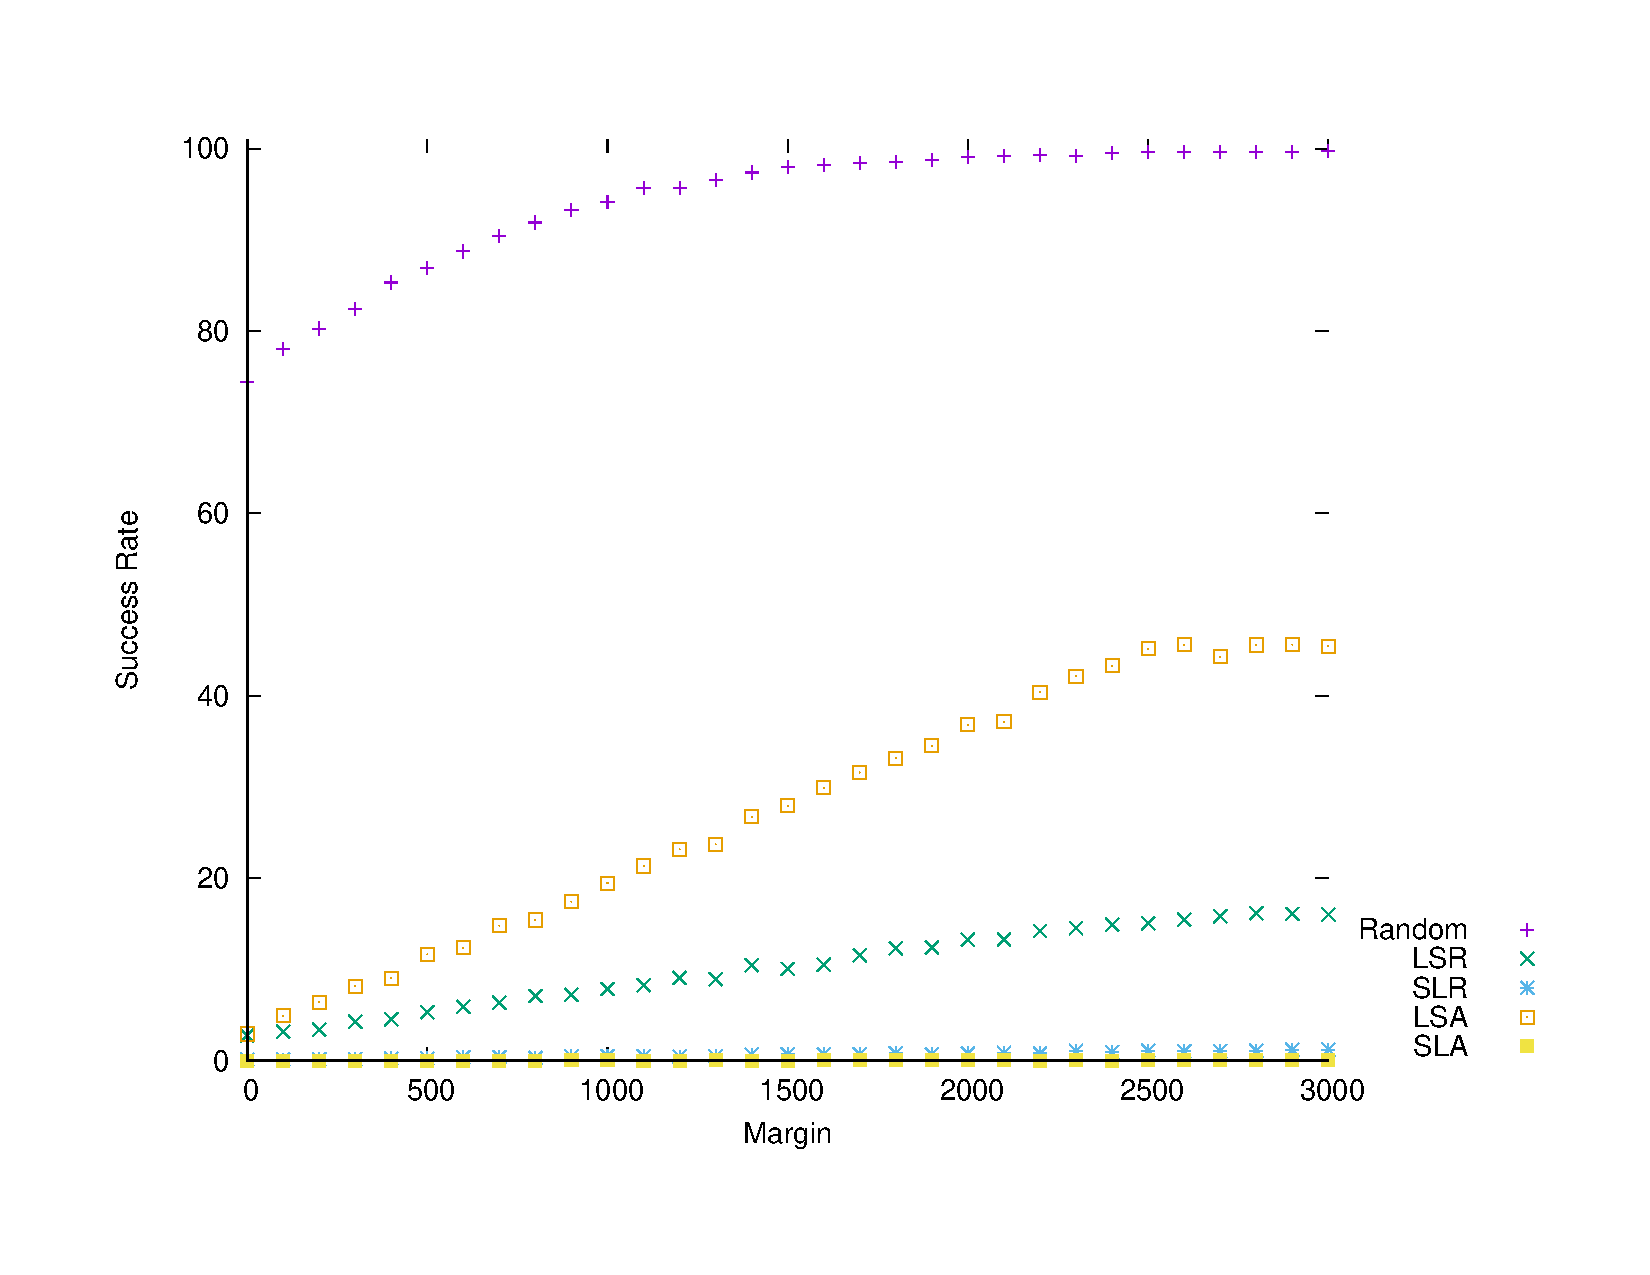
\includegraphics[scale=0.4]{departs_gp_21000.pdf}
      \end{center}
      \caption{Success rate of the sending orders for $P = 21000$}
      
     \end{figure}
     
     
       
\begin{figure}[H] 

       \begin{center}
      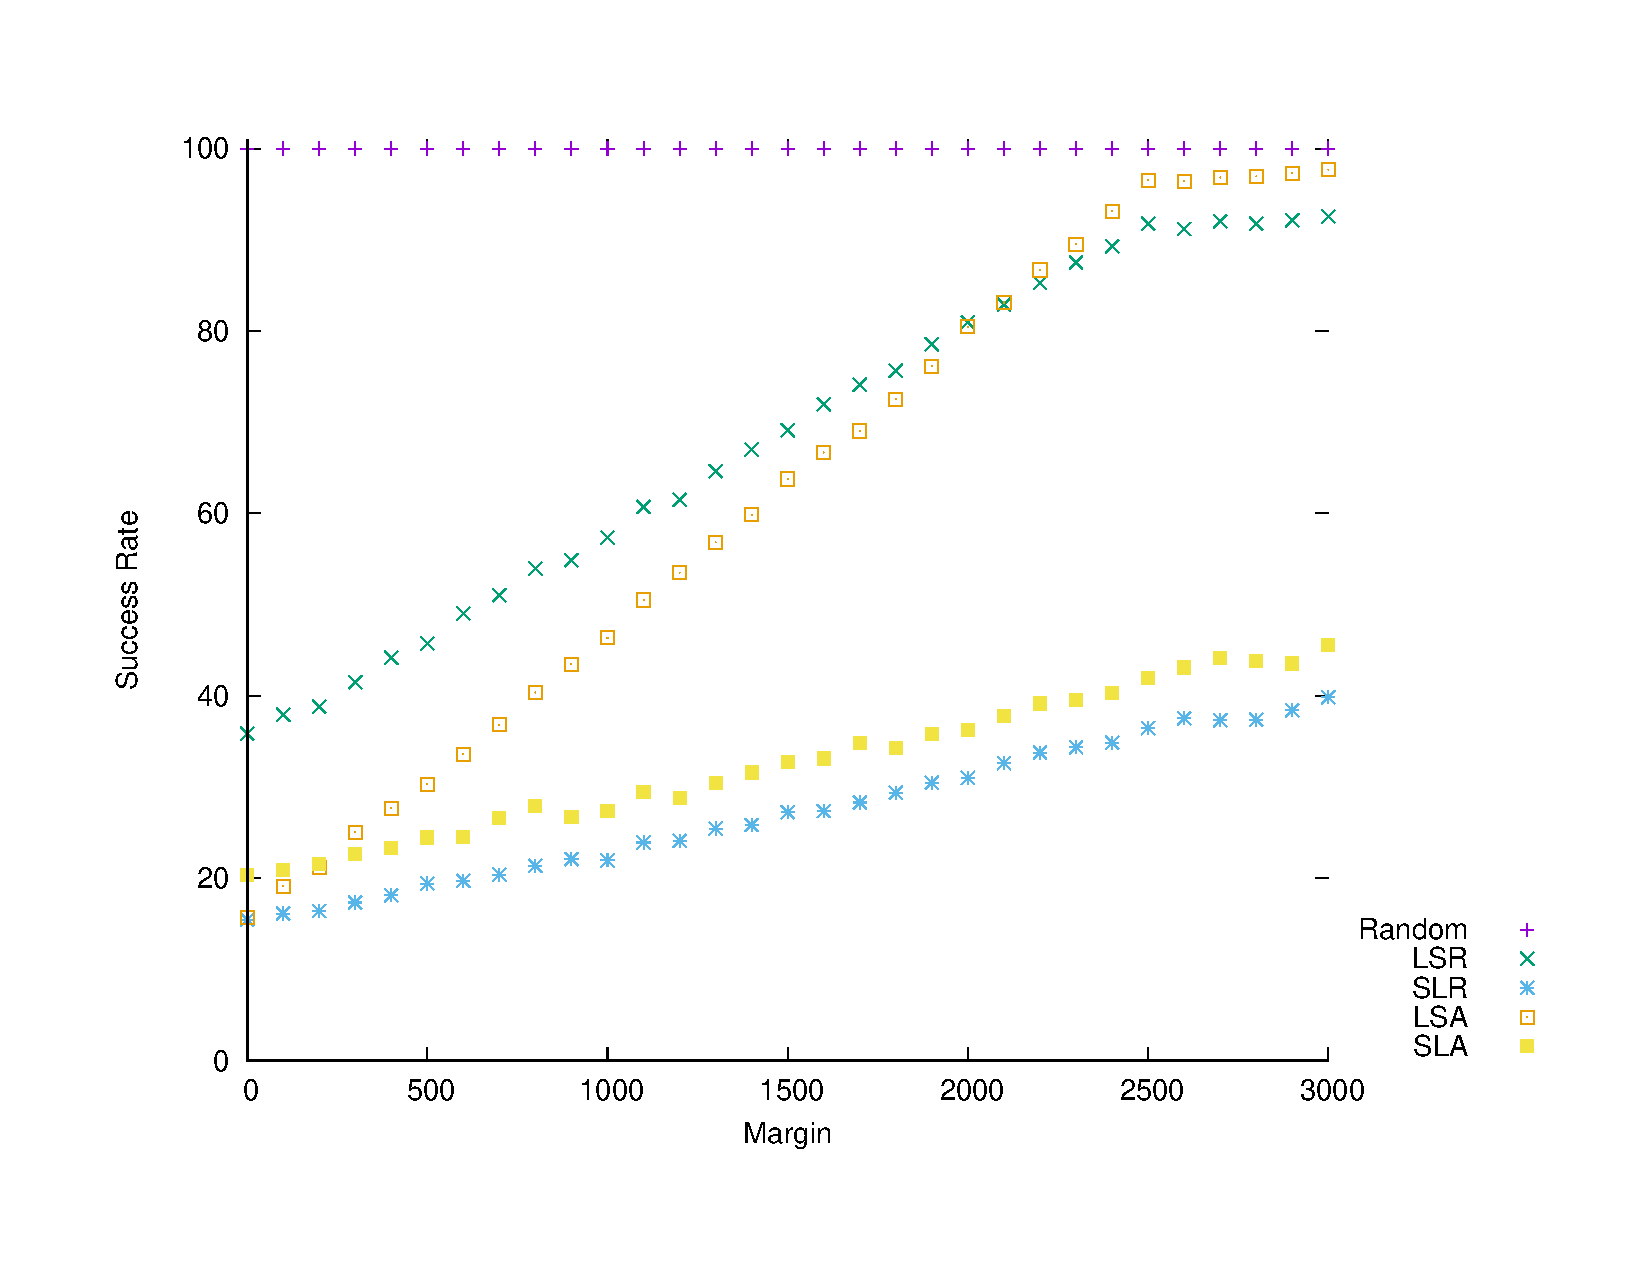
\includegraphics[scale=0.4]{departs_gp_30000.pdf}
      \end{center}
      \caption{Success rate of the sending orders for a $P = 30000$}
      \label{fig:success30000}
     \end{figure}
     
     First, we remark that, for every sending order, the success rate is strictly better for large periods. This is due to the fact that the size of the period is a factor for failure. According to our results, the two SL sending orders are not good, in any cases. However, the LS orders seem to increase when the flexibility is large enough, but in the two regimes, they appear to be stagnating to a lower success rate than Random. As we can see the random finds near to 100\% of the solutions when the period is large enough, even when we give no flexibility. 
     %On average, it is necessary to draw 6 randoms sending order to find a solution, when the period is large, but in some particularly hard instances, it can be impossible to find a solution, even with 100 randoms sending orders. 
     
     To observe  the impact of the number of random sending orders drawn, we compared the success rate of the following number of drawing, on graphs in which the links are drawn  between $0$ and $20000$ slots, with a period $P=20000$, and a flexibility of $0$. The following table present the average success rate of each number of sending orders, on $1000$ instances.
       \begin{figure}[H] 

       \begin{center}
   \begin{tabular}{|c|c|c|c|c|c|c|}
    \hline
    number of randoms & $1$ & $10$ & $100$& $1 000$& $10 000$&$100 000$\\
    \hline
    Success rate $(\simeq)$ & $17,8$ &$60,5$&$77,7$&$80,5$&$80,5$&$80,5$\\
    \hline
      \end{tabular}
      \end{center}
   \caption{Impact of the number of randoms sending orders drawn}
     \end{figure}
     
     In our case of $8$ routes, the number of different possible sending orders is $8! \simeq 40 000$. By drawing $1000$ random sending orders, we explore near to $2,5 \%$ of the cases, which seems enough to find as many solutions as if generate more random sending orders.

     

     We now want to compare the performances of the different algorithms on the way back. Since GP showed some excellent results on large periods (see Fig~\ref{fig:success30000}), it is more interesting to focus on the behavior of the algorithms on short periods. The following experience is realized on graph with $8$ routes (links between $0$ and $20000$), and with a period of $21000$. Since we just conclude that drawing $1000$ sending order is enough, with $8$ routes, we now generate $1000$ randoms sending orders instead of $100$.
     

 
    \begin{figure} [H] 
       \begin{center}
      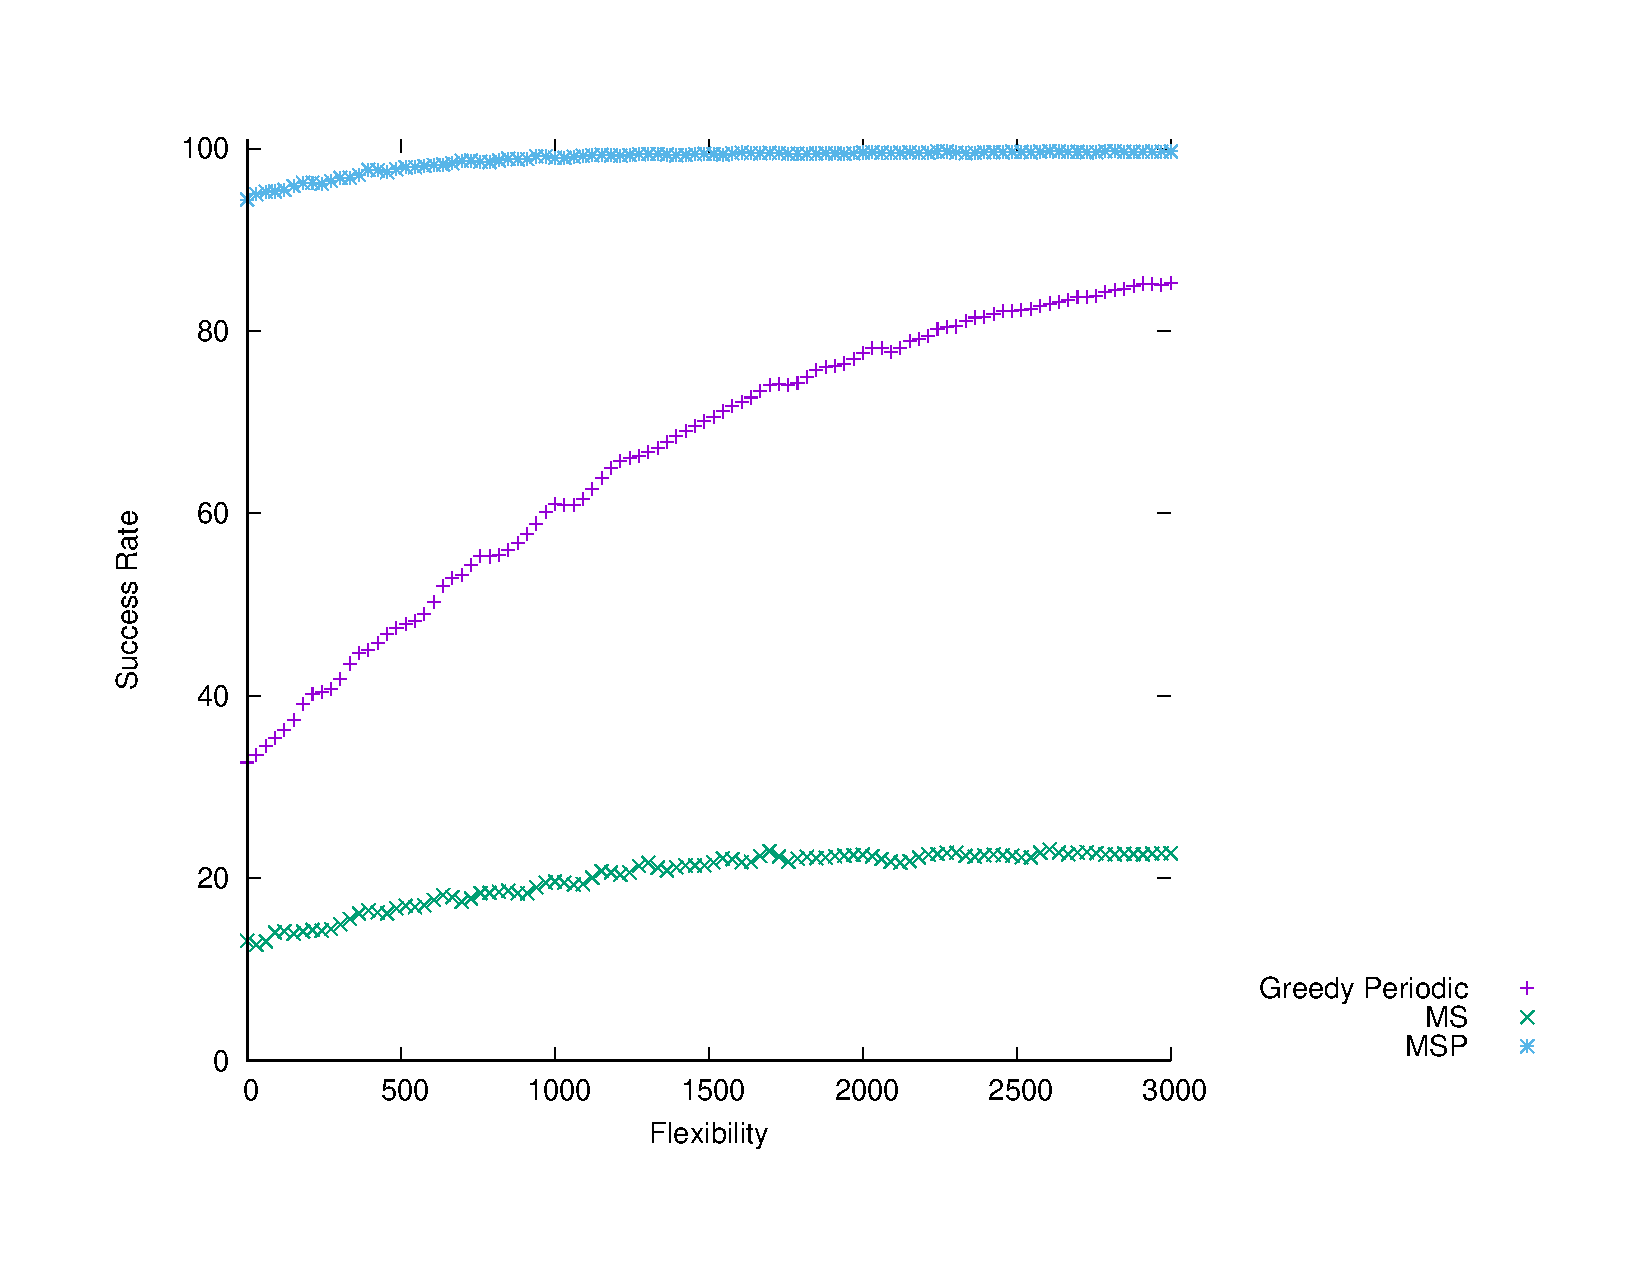
\includegraphics[scale=0.4]{retour_21000.pdf}
      \end{center}
      \caption{Success rate of the different algorithms for a $P = 21000$}
     \label{fig:success21000}
     \end{figure}
     
     The algorithm MS, that does not consider the periodicity for the scheduling is far worst than the others, and, even if GP seems to converge too $100\%$ of success rate when the flexibility is large enough, MSP is always strictly better. We remark that when the flexibility is low ($<500$) there is still near to $5\%$ of failure for MSP. 
   
   Thus, using the Random sending order combined with MSP for the way back seems to be a very good algorithm to solve PALL. Nevertheless, there is still a few number of instances in the worst area of parameters (very short period, and very low flexibility), that are impossible to solve with our algorithm.
     

 To evaluate the performance of our best algorithm to find solutions, that is, generating $1000$ randoms sending orders and using MSP on the way back, we compared it's performance against the actual way to manage the messages in a network. Nowadays, the networks are managed through a stochastic model. The messages in the nodes are assigned following a FIFO rule. Even if this policy works well, in practice when the network is not too loaded, it does not ensure a minimum latency. Thus, some latency critical applications like C-RAN needs some deterministic algorithms. To model such a network, we generate some randoms offsets in the sources. Then we simulate the behavior of a stochastic network during a great number of periods.
 
We simulated a stochastic network on $1000$ instances with $8$ long routes (links between $0$ and $20000$). The results are not really different if we use short routes. The flexibility needed by an instance of the network is computed by taking the message which have the highest process time, at which we subtract the weight of the longest route. We measure, for periods from $20000$ ( network fully loaded), to $50000$ ($40 \%$ of load), the medians, the first, and the third quartiles of $1000$ results.
     
      
    \begin{figure}[H] 

       \begin{center}
     % 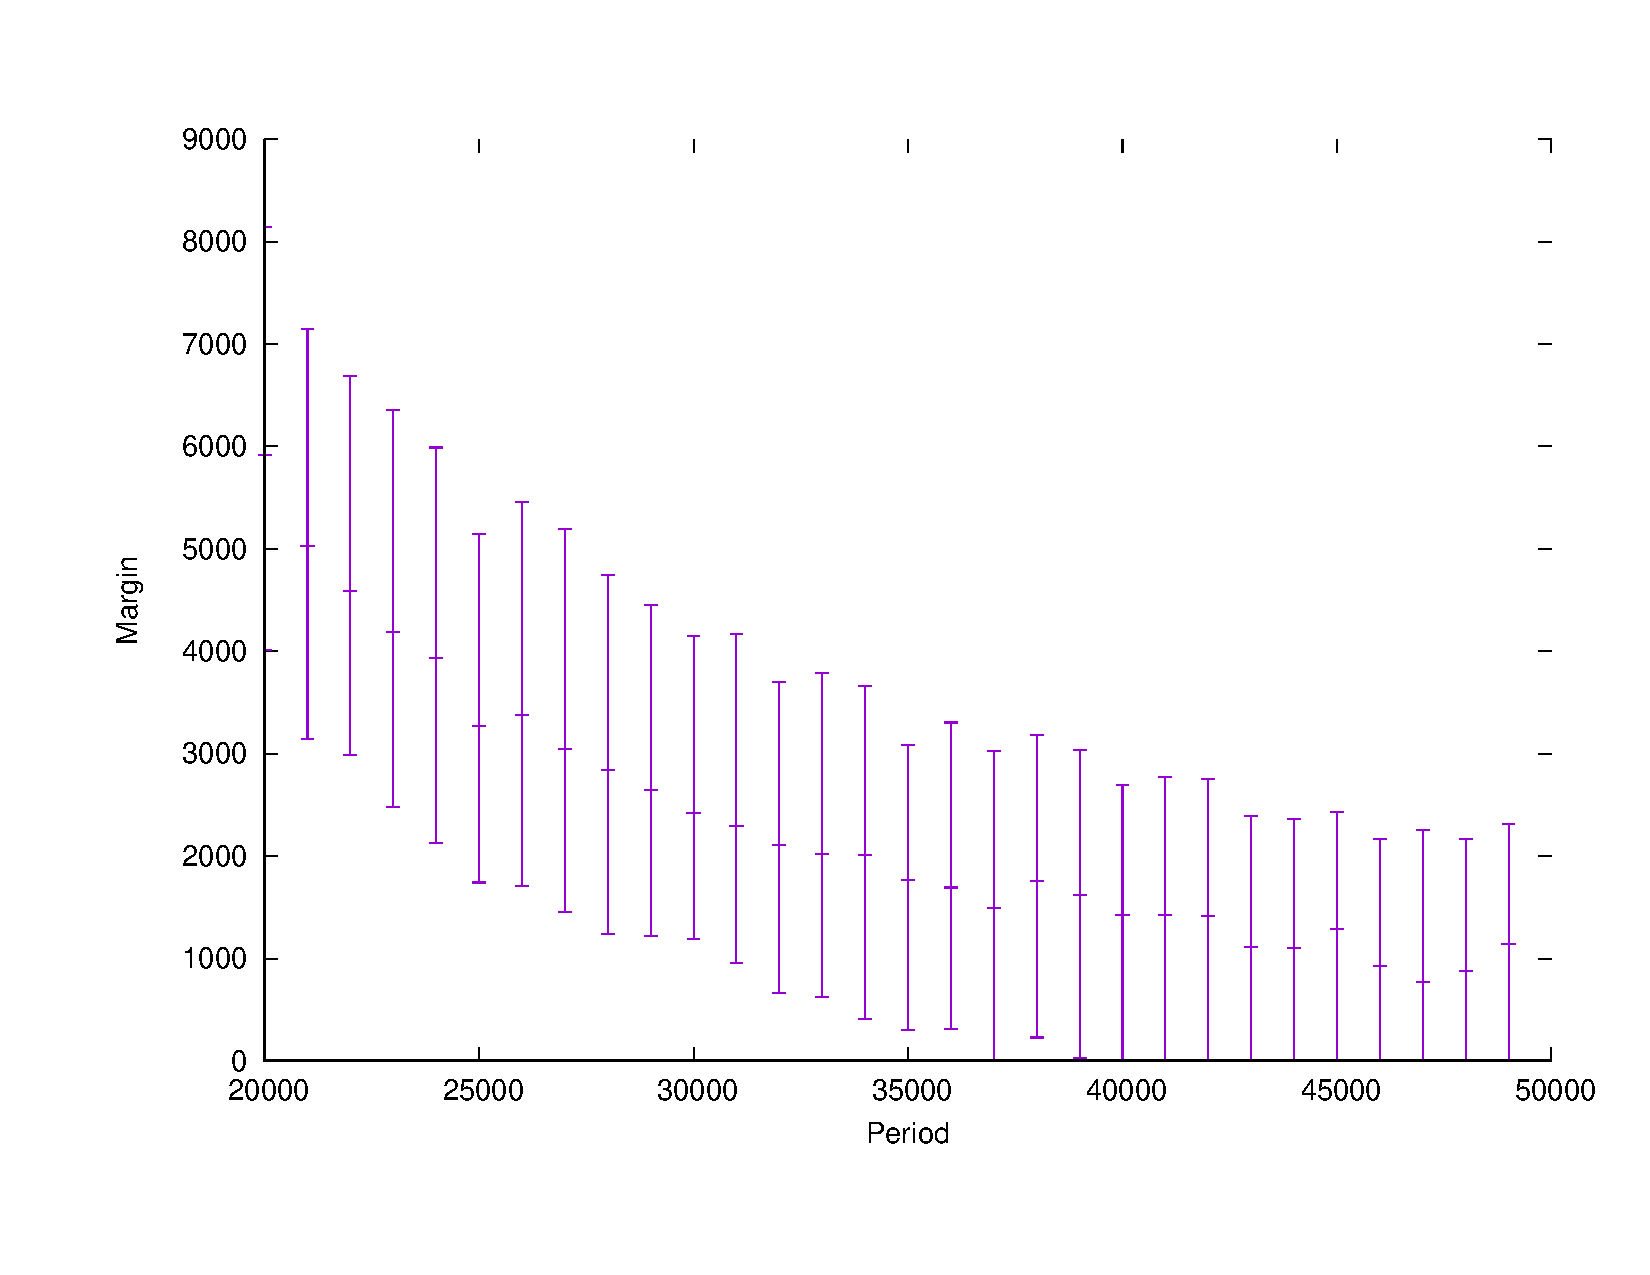
\includegraphics[scale=0.4]{stochastic.pdf}
       % GNUPLOT: LaTeX picture
\setlength{\unitlength}{0.240900pt}
\ifx\plotpoint\undefined\newsavebox{\plotpoint}\fi
\sbox{\plotpoint}{\rule[-0.200pt]{0.400pt}{0.400pt}}%
\begin{picture}(1500,900)(0,0)
\sbox{\plotpoint}{\rule[-0.200pt]{0.400pt}{0.400pt}}%
\put(171.0,131.0){\rule[-0.200pt]{4.818pt}{0.400pt}}
\put(151,131){\makebox(0,0)[r]{$0$}}
\put(1279.0,131.0){\rule[-0.200pt]{4.818pt}{0.400pt}}
\put(171.0,212.0){\rule[-0.200pt]{4.818pt}{0.400pt}}
\put(151,212){\makebox(0,0)[r]{$1000$}}
\put(1279.0,212.0){\rule[-0.200pt]{4.818pt}{0.400pt}}
\put(171.0,293.0){\rule[-0.200pt]{4.818pt}{0.400pt}}
\put(151,293){\makebox(0,0)[r]{$2000$}}
\put(1279.0,293.0){\rule[-0.200pt]{4.818pt}{0.400pt}}
\put(171.0,374.0){\rule[-0.200pt]{4.818pt}{0.400pt}}
\put(151,374){\makebox(0,0)[r]{$3000$}}
\put(1279.0,374.0){\rule[-0.200pt]{4.818pt}{0.400pt}}
\put(171.0,455.0){\rule[-0.200pt]{4.818pt}{0.400pt}}
\put(151,455){\makebox(0,0)[r]{$4000$}}
\put(1279.0,455.0){\rule[-0.200pt]{4.818pt}{0.400pt}}
\put(171.0,535.0){\rule[-0.200pt]{4.818pt}{0.400pt}}
\put(151,535){\makebox(0,0)[r]{$5000$}}
\put(1279.0,535.0){\rule[-0.200pt]{4.818pt}{0.400pt}}
\put(171.0,616.0){\rule[-0.200pt]{4.818pt}{0.400pt}}
\put(151,616){\makebox(0,0)[r]{$6000$}}
\put(1279.0,616.0){\rule[-0.200pt]{4.818pt}{0.400pt}}
\put(171.0,697.0){\rule[-0.200pt]{4.818pt}{0.400pt}}
\put(151,697){\makebox(0,0)[r]{$7000$}}
\put(1279.0,697.0){\rule[-0.200pt]{4.818pt}{0.400pt}}
\put(171.0,778.0){\rule[-0.200pt]{4.818pt}{0.400pt}}
\put(151,778){\makebox(0,0)[r]{$8000$}}
\put(1279.0,778.0){\rule[-0.200pt]{4.818pt}{0.400pt}}
\put(171.0,859.0){\rule[-0.200pt]{4.818pt}{0.400pt}}
\put(151,859){\makebox(0,0)[r]{$9000$}}
\put(1279.0,859.0){\rule[-0.200pt]{4.818pt}{0.400pt}}
\put(171.0,131.0){\rule[-0.200pt]{0.400pt}{4.818pt}}
\put(171,90){\makebox(0,0){$20000$}}
\put(171.0,839.0){\rule[-0.200pt]{0.400pt}{4.818pt}}
\put(359.0,131.0){\rule[-0.200pt]{0.400pt}{4.818pt}}
\put(359,90){\makebox(0,0){$25000$}}
\put(359.0,839.0){\rule[-0.200pt]{0.400pt}{4.818pt}}
\put(547.0,131.0){\rule[-0.200pt]{0.400pt}{4.818pt}}
\put(547,90){\makebox(0,0){$30000$}}
\put(547.0,839.0){\rule[-0.200pt]{0.400pt}{4.818pt}}
\put(735.0,131.0){\rule[-0.200pt]{0.400pt}{4.818pt}}
\put(735,90){\makebox(0,0){$35000$}}
\put(735.0,839.0){\rule[-0.200pt]{0.400pt}{4.818pt}}
\put(923.0,131.0){\rule[-0.200pt]{0.400pt}{4.818pt}}
\put(923,90){\makebox(0,0){$40000$}}
\put(923.0,839.0){\rule[-0.200pt]{0.400pt}{4.818pt}}
\put(1111.0,131.0){\rule[-0.200pt]{0.400pt}{4.818pt}}
\put(1111,90){\makebox(0,0){$45000$}}
\put(1111.0,839.0){\rule[-0.200pt]{0.400pt}{4.818pt}}
\put(1299.0,131.0){\rule[-0.200pt]{0.400pt}{4.818pt}}
\put(1299,90){\makebox(0,0){$50000$}}
\put(1299.0,839.0){\rule[-0.200pt]{0.400pt}{4.818pt}}
\put(171.0,131.0){\rule[-0.200pt]{0.400pt}{175.375pt}}
\put(171.0,131.0){\rule[-0.200pt]{271.735pt}{0.400pt}}
\put(30,495){\makebox(0,0){Needed Flexibility}}
\put(735,29){\makebox(0,0){Period}}
\put(171.0,455.0){\rule[-0.200pt]{0.400pt}{81.183pt}}
\put(171.0,455.0){\rule[-0.200pt]{2.409pt}{0.400pt}}
\put(171.0,792.0){\rule[-0.200pt]{2.409pt}{0.400pt}}
\put(209.0,412.0){\rule[-0.200pt]{0.400pt}{73.715pt}}
\put(199.0,412.0){\rule[-0.200pt]{4.818pt}{0.400pt}}
\put(199.0,718.0){\rule[-0.200pt]{4.818pt}{0.400pt}}
\put(246.0,353.0){\rule[-0.200pt]{0.400pt}{79.497pt}}
\put(236.0,353.0){\rule[-0.200pt]{4.818pt}{0.400pt}}
\put(236.0,683.0){\rule[-0.200pt]{4.818pt}{0.400pt}}
\put(284.0,336.0){\rule[-0.200pt]{0.400pt}{75.883pt}}
\put(274.0,336.0){\rule[-0.200pt]{4.818pt}{0.400pt}}
\put(274.0,651.0){\rule[-0.200pt]{4.818pt}{0.400pt}}
\put(321.0,306.0){\rule[-0.200pt]{0.400pt}{70.343pt}}
\put(311.0,306.0){\rule[-0.200pt]{4.818pt}{0.400pt}}
\put(311.0,598.0){\rule[-0.200pt]{4.818pt}{0.400pt}}
\put(359.0,297.0){\rule[-0.200pt]{0.400pt}{73.715pt}}
\put(349.0,297.0){\rule[-0.200pt]{4.818pt}{0.400pt}}
\put(349.0,603.0){\rule[-0.200pt]{4.818pt}{0.400pt}}
\put(397.0,270.0){\rule[-0.200pt]{0.400pt}{63.598pt}}
\put(387.0,270.0){\rule[-0.200pt]{4.818pt}{0.400pt}}
\put(387.0,534.0){\rule[-0.200pt]{4.818pt}{0.400pt}}
\put(434.0,269.0){\rule[-0.200pt]{0.400pt}{64.561pt}}
\put(424.0,269.0){\rule[-0.200pt]{4.818pt}{0.400pt}}
\put(424.0,537.0){\rule[-0.200pt]{4.818pt}{0.400pt}}
\put(472.0,238.0){\rule[-0.200pt]{0.400pt}{69.138pt}}
\put(462.0,238.0){\rule[-0.200pt]{4.818pt}{0.400pt}}
\put(462.0,525.0){\rule[-0.200pt]{4.818pt}{0.400pt}}
\put(509.0,226.0){\rule[-0.200pt]{0.400pt}{62.393pt}}
\put(499.0,226.0){\rule[-0.200pt]{4.818pt}{0.400pt}}
\put(499.0,485.0){\rule[-0.200pt]{4.818pt}{0.400pt}}
\put(547.0,222.0){\rule[-0.200pt]{0.400pt}{60.225pt}}
\put(537.0,222.0){\rule[-0.200pt]{4.818pt}{0.400pt}}
\put(537.0,472.0){\rule[-0.200pt]{4.818pt}{0.400pt}}
\put(585.0,195.0){\rule[-0.200pt]{0.400pt}{60.225pt}}
\put(575.0,195.0){\rule[-0.200pt]{4.818pt}{0.400pt}}
\put(575.0,445.0){\rule[-0.200pt]{4.818pt}{0.400pt}}
\put(622.0,185.0){\rule[-0.200pt]{0.400pt}{58.780pt}}
\put(612.0,185.0){\rule[-0.200pt]{4.818pt}{0.400pt}}
\put(612.0,429.0){\rule[-0.200pt]{4.818pt}{0.400pt}}
\put(660.0,178.0){\rule[-0.200pt]{0.400pt}{59.743pt}}
\put(650.0,178.0){\rule[-0.200pt]{4.818pt}{0.400pt}}
\put(650.0,426.0){\rule[-0.200pt]{4.818pt}{0.400pt}}
\put(697.0,188.0){\rule[-0.200pt]{0.400pt}{59.020pt}}
\put(687.0,188.0){\rule[-0.200pt]{4.818pt}{0.400pt}}
\put(687.0,433.0){\rule[-0.200pt]{4.818pt}{0.400pt}}
\put(735.0,152.0){\rule[-0.200pt]{0.400pt}{55.889pt}}
\put(725.0,152.0){\rule[-0.200pt]{4.818pt}{0.400pt}}
\put(725.0,384.0){\rule[-0.200pt]{4.818pt}{0.400pt}}
\put(773.0,146.0){\rule[-0.200pt]{0.400pt}{57.575pt}}
\put(763.0,146.0){\rule[-0.200pt]{4.818pt}{0.400pt}}
\put(763.0,385.0){\rule[-0.200pt]{4.818pt}{0.400pt}}
\put(810.0,146.0){\rule[-0.200pt]{0.400pt}{54.925pt}}
\put(800.0,146.0){\rule[-0.200pt]{4.818pt}{0.400pt}}
\put(800.0,374.0){\rule[-0.200pt]{4.818pt}{0.400pt}}
\put(848.0,143.0){\rule[-0.200pt]{0.400pt}{56.371pt}}
\put(838.0,143.0){\rule[-0.200pt]{4.818pt}{0.400pt}}
\put(838.0,377.0){\rule[-0.200pt]{4.818pt}{0.400pt}}
\put(885.0,140.0){\rule[-0.200pt]{0.400pt}{56.371pt}}
\put(875.0,140.0){\rule[-0.200pt]{4.818pt}{0.400pt}}
\put(875.0,374.0){\rule[-0.200pt]{4.818pt}{0.400pt}}
\put(923.0,133.0){\rule[-0.200pt]{0.400pt}{54.202pt}}
\put(913.0,133.0){\rule[-0.200pt]{4.818pt}{0.400pt}}
\put(913.0,358.0){\rule[-0.200pt]{4.818pt}{0.400pt}}
\put(961.0,131.0){\rule[-0.200pt]{0.400pt}{55.166pt}}
\put(951.0,131.0){\rule[-0.200pt]{4.818pt}{0.400pt}}
\put(951.0,360.0){\rule[-0.200pt]{4.818pt}{0.400pt}}
\put(998.0,131.0){\rule[-0.200pt]{0.400pt}{49.384pt}}
\put(988.0,131.0){\rule[-0.200pt]{4.818pt}{0.400pt}}
\put(988.0,336.0){\rule[-0.200pt]{4.818pt}{0.400pt}}
\put(1036.0,131.0){\rule[-0.200pt]{0.400pt}{48.180pt}}
\put(1026.0,131.0){\rule[-0.200pt]{4.818pt}{0.400pt}}
\put(1026.0,331.0){\rule[-0.200pt]{4.818pt}{0.400pt}}
\put(1073.0,131.0){\rule[-0.200pt]{0.400pt}{47.216pt}}
\put(1063.0,131.0){\rule[-0.200pt]{4.818pt}{0.400pt}}
\put(1063.0,327.0){\rule[-0.200pt]{4.818pt}{0.400pt}}
\put(1111.0,131.0){\rule[-0.200pt]{0.400pt}{46.975pt}}
\put(1101.0,131.0){\rule[-0.200pt]{4.818pt}{0.400pt}}
\put(1101.0,326.0){\rule[-0.200pt]{4.818pt}{0.400pt}}
\put(1149.0,131.0){\rule[-0.200pt]{0.400pt}{45.048pt}}
\put(1139.0,131.0){\rule[-0.200pt]{4.818pt}{0.400pt}}
\put(1139.0,318.0){\rule[-0.200pt]{4.818pt}{0.400pt}}
\put(1186.0,131.0){\rule[-0.200pt]{0.400pt}{46.494pt}}
\put(1176.0,131.0){\rule[-0.200pt]{4.818pt}{0.400pt}}
\put(1176.0,324.0){\rule[-0.200pt]{4.818pt}{0.400pt}}
\put(1224.0,131.0){\rule[-0.200pt]{0.400pt}{45.048pt}}
\put(1214.0,131.0){\rule[-0.200pt]{4.818pt}{0.400pt}}
\put(1214.0,318.0){\rule[-0.200pt]{4.818pt}{0.400pt}}
\put(1261.0,131.0){\rule[-0.200pt]{0.400pt}{41.194pt}}
\put(1251.0,131.0){\rule[-0.200pt]{4.818pt}{0.400pt}}
\put(171,608){\makebox(0,0){$+$}}
\put(209,562){\makebox(0,0){$+$}}
\put(246,503){\makebox(0,0){$+$}}
\put(284,479){\makebox(0,0){$+$}}
\put(321,431){\makebox(0,0){$+$}}
\put(359,429){\makebox(0,0){$+$}}
\put(397,390){\makebox(0,0){$+$}}
\put(434,382){\makebox(0,0){$+$}}
\put(472,367){\makebox(0,0){$+$}}
\put(509,340){\makebox(0,0){$+$}}
\put(547,327){\makebox(0,0){$+$}}
\put(585,317){\makebox(0,0){$+$}}
\put(622,307){\makebox(0,0){$+$}}
\put(660,302){\makebox(0,0){$+$}}
\put(697,300){\makebox(0,0){$+$}}
\put(735,278){\makebox(0,0){$+$}}
\put(773,273){\makebox(0,0){$+$}}
\put(810,268){\makebox(0,0){$+$}}
\put(848,267){\makebox(0,0){$+$}}
\put(885,254){\makebox(0,0){$+$}}
\put(923,248){\makebox(0,0){$+$}}
\put(961,259){\makebox(0,0){$+$}}
\put(998,234){\makebox(0,0){$+$}}
\put(1036,234){\makebox(0,0){$+$}}
\put(1073,232){\makebox(0,0){$+$}}
\put(1111,228){\makebox(0,0){$+$}}
\put(1149,216){\makebox(0,0){$+$}}
\put(1186,212){\makebox(0,0){$+$}}
\put(1224,227){\makebox(0,0){$+$}}
\put(1261,203){\makebox(0,0){$+$}}
\put(1251.0,302.0){\rule[-0.200pt]{4.818pt}{0.400pt}}
\put(171.0,131.0){\rule[-0.200pt]{0.400pt}{175.375pt}}
\put(171.0,131.0){\rule[-0.200pt]{271.735pt}{0.400pt}}
\end{picture}

      \end{center}
      \caption{Needed flexibility on stochastic networks according to the load.}
      \label{fig:sto}
     \end{figure}
     
     
    We also made a linear search to find the minimum flexibility needed by our algorithm on those loads to find a solution. There are few cases, when both the flexibility and the period are too restricted in which there is no solutions: with a period of $20000$, our algorithm needs in average $\simeq 80$ slots of flexibility to find a solution. Otherwise, the algorithm finds a solution with $0$ flexibility for every periods $>20000$. On the other hand, the stochastic policy does not ensure a minimal latency. As we can see in Fig~\ref{fig:sto}), the more the network is loaded, the higher the latency is. Even if the first quartile is to $0$ when the network is not highly loaded, many instances needs some flexibility. Moreover, the latency is not guaranteed with that policy. Indeed, even if half of the cases of our simulations works with less than $1000$ slots of flexibility on a light loaded network, that could be reasonable for specific applications, $25\%$ of the cases needs more than $2000$ slots of flexibility. With our algorithm, we control the latency, and here, we have optimal solutions that makes it really appropriate.

    
    \paragraph*{Future works}
   
   We plan to generalize our study of the PALL problem to more topologies,
   such as trees and cycles which are commonly found in real networks. 
   We would like to design FPT algorithms in the number of routes for PAZL and PALL on the star topology, eventually by relaxing the constraint on the maximal process time into an constraint on the average process time, which seems much more tractable. 
   Moreoever we could allow preemption, that is the messages are allowed to be cut into pieces,
   which would certainly change the complexity of the problem. 
   Finally, the routes may not be fixed but chosen to optimize the latency, which would make the problem even more difficult (maybe $\Pi_2$-complete instead of $\NP$-complete). 

   


\bibliographystyle{ieeetr}
\bibliography{Sources}

\end{document}
